%: ----------------------- introduction file header -----------------------
\begin{savequote}[50mm]
So you see, the only proof of what you are is in the way you hear the truth.
% Don't be scared, live to win, although they're always gonna tell you it's a sin.
\qauthor{Motörhead}
\end{savequote}

% the code below specifies where the figures are stored
\ifpdf
\graphicspath{{5_experiments_and_results/figures/PNG/}
{5_experiments_and_results/figures/PDF/}{5_experiments_and_results/figures/}}
\fi

\chapter{Evaluation}
\label{cha:evaluation}
%------------------------------------------------------------------------- 

% INTRODUCTION OF THE CHAPTER

In the previous chapters several contributions have been presented. All these
contributions together define AdaptUI, a mobile platform which tackles adaptive 
and dynamic user interfacing for mobile devices. AdaptUI combines mobile 
semantics and reasoning, supported by an ontology which models user's 
characteristics, context current conditions and device's hardware and software 
characteristics. In this chapter an evaluation of the designed ontology and the 
semantic based platform which manages it is performed. This evaluation is 
addressed through several quantitative experiments regarding system performance 
with specific operations (e.g., reasoning over a controlled set of rules), other 
alternatives to adaptive user interfacing and, finally, analysing users' 
acceptance and feedback.

Consequently, this chapter is divided in two different parts considering the 
experiments' goals. On one hand, an evaluation of the technical performance
of the AdaptUI system is presented. This evaluation includes quantitative and 
qualitative experiments. It has been developed as follows:

\begin{enumerate}[label=\alph*)]
  \item First, the developed mobile adaptation of the Pellet reasoning engine 
  is tested through several scenarios. In these scenarios different modifications 
  of the AdaptUIOnt ontology are presented in order to evaluate the performance 
  differences between \textit{Pellet4Android} and Pellet when dealing with different
  designed ontologies.
  
  \item Secondly, as the system's goal is to adapt the user interface, a comparison 
  with another user interface adaptation solution has been performed: the 
  Imhotep framework. Imhotep is a user interface adaptation framework which 
  aims to ease the development of adaptable and more accessible user interfaces.
%   ,
%   and it is also the beginning of the experience we have in the user interface
%   adaptation field.
  
  \item Next, several scenarios are presented in which the adaptation process
  of the AdaptUI system is described step by step, from the scenario conditions
  to the adaptation results. These scenarios have been divided into three 
  different groups, each group aiming to cover different types of adaptation 
  and environments. This classification includes:
  \begin{itemize}
    \item A scenario in which the limitations suffered by the user are caused
    by the current context conditions. 
    
    \item A second scenario introducing several limitations due to the  
    activities the user performs.
    
    \item A final case in which several disabilities imped the user to interact 
    properly with the user interface.
  \end{itemize}
  
  \item Finally, the \acp{api} that AdaptUI provides are tested with Android
  developers. The participating developers have to deal with the twofold purpose
  of the AdaptUI \ac{api}. On the one hand, developers are requested to modify
  the knowledge represented in a test version of the AdaptUIOnt ontology. On the
  other hand, they have to implement an adaptive user interface in Android.
\end{enumerate}

Besides, an evaluation including actual users, without technical knowledge
requisites, is performed. This part of the evaluation is based on their user
satisfaction when using AdaptUI. The scenario for this experiment includes the
user and an Android based tutorial through which the user calibrates several 
interaction parameters. Taking into account different context situations, several 
applications are adapted consequently. After the adaptation, the user is 
requested to complete a questionnaire of usability. More concretely, the \ac{sus} 
questionnaire is presented (among several extra questions to classify the 
results).

Hence, the reminder of this chapter has been structured as follows: 

\begin{itemize}
  \item A technical evaluation, whose experiments are detailed in 
  Section~\ref{sec:technical_evaluation}. These experiments assess the 
  reasoning performance comparing Pellet for desktop versus Pellet for mobile 
  devices. The provided \acp{api} have been also evaluated in an experiment
  including developers. AdaptUI aims to perform all the adaptations in the
  mobile device. Besides, the designed models have been developed using semantics,
  together with a set of rules which manages the process. Thus, a remarkable
  part of the whole AdaptUI architecture is \textit{Pellet4Android}, the Android
  version of Pellet included in the Adaptation Engine (see Section~\ref{sec:semantic_modeller}).
  Hence, this part of the evaluation includes the corresponding comparison of
  both Pellet versions.
  
  \item A usability evaluation of the system, whose details are accordingly 
  described in Section~\ref{sec:user_evaluation}. This evaluation includes 
  users interacting with the AdaptUI system. In order to evaluate the usability 
  of AdaptUI the \ac{sus}, a usability questionnaire, is presented to the users. 
  Section~\ref{sec:sus_results} presents Table~\ref{tbl:additional_questions} and
  Table~\ref{tbl:sus_questionnaire_results}, which shows the responses from all
  the users participating in the evaluation of AdaptUI.

  \item Finally, Section~\ref{sec:evaluation_discussion} and 
  Section~\ref{sec:evaluation_conclusions} summarize and analyse the results
  obtained and detailed in the previous sections, regarding both technical and
  usability aspects.
\end{itemize}

\section{Technical Evaluation}
\label{sec:technical_evaluation}

The technical evaluation of this chapter includes several experiments that are 
carried out aiming to test the performance of the adaptation process. One of 
the most important developed modules of AdaptUI is the Pellet reasoning 
engine port for Android. This module requires special emphasis in the evaluation, 
as leads the whole adaptation process. Besides, several other experiments are 
presented. Thus, in the following sections these experiments and their results 
are detailed:

% This section gathers several experiments regarding the technical part of the 
% evaluation. Within this section the following experiments are included:

\begin{enumerate}[label=\alph*)]
  \item First, Section~\ref{sec:performance_evaluation} presents a series 
  of experiments regarding the performance of \textit{Pellet4Android} in 
  comparison with Pellet for Java. These experiments include the default
  AdaptUIOnt ontology and different versions of AdaptUIOnt with several modifications
  of the axioms sets. For more details of the \textit{Pellet4Android} mobile 
  reasoning engine see Section~\ref{sec:pellet4android}.
  
  \item Second, AdaptUI is compared to another user adaptation solution: 
  Imhotep. This is detailed in Section~\ref{sec:imhotep_comparison}.
  
  \item Next, several scenarios are presented to evaluate the adaptation 
  process of AdaptUI. Besides, a comparison with Imhotep user adaptation 
  framework is also performed. The scenarios and their details are given in 
  Section~\ref{sec:scenarios}.
  
  \item Finally, $5$ developers with experience in developing Android based 
  applications have evaluated the provided \acs{api}. This experiment is detailed
  in Section~\ref{sec:developers}.
\end{enumerate}


\subsection{Performance Evaluation for Pellet and Pellet4Android}
\label{sec:performance_evaluation}

During this section different experiments are presented in order to 
discuss the results of using mobile reasoning engines. In our case we evaluate 
the reasoning performance of \textit{Pellet4Android}, the Android based version 
of Pellet ported for AdaptUI. To do so, this evaluation considers Pellet, the 
desktop Java based reasoning engine, to make a comparison between the 
performance results of both solutions. This evaluation has been divided into 
three different experiments:

\begin{enumerate}
  \item The first experiment consists in using the default AdaptUIOnt ontology 
  version with both reasoning engines. When loading the ontology several rules 
  are processed and triggered. As a result of this experiment the  
  corresponding performance results are compared.
  
  \item For the second experiment the ABox axioms set of the AdaptUIOnt 
  ontology is increased. The ABox gathers the knowledge about the 
  individuals, including concepts and roles assertions, and individuals 
  equality and inequality~\citep{krotzsch_description_2012}. In other words, 
  it describes the attributes of instances (or individuals), the roles between 
  instances, and other assertions about instances regarding their class 
  membership with the TBox concepts~\citep{abox_tbox}. The ABox, RBox and TBox 
  belong to the \ac{owl} 2 Description Logic (DL). As for these experiments several 
  modifications have been carried out in these axiom sets, a more concrete 
  description of the concepts represented by each set is detailed in 
  Table~\ref{tbl:dl_terminology}. Hence, increasing the number of individuals   
  might result into difference performance results comparing both platforms.
  
  \item Next, the \ac{swrl} axioms set of the AdaptUIOnt ontology is modified by 
  increasing its axioms. This axiom set collects axioms related to the rules 
  included in the ontology. Therefore, this experiment focuses on the reasoning 
  capabilities of each version of Pellet.
\end{enumerate}

\begin{table}
 \caption{TBox and ABox components purposes~\citep{abox_tbox}.}
 \label{tbl:dl_terminology}
 \footnotesize
 \centering
\begin{tabular}{l l l}
  \hline 
  \textbf{ABox} 				&  \textbf{TBox} \\
  \hline 
  Membership assertions, either as concepts or  & Definitions of the concepts and properties of the 	\\
  as roles. 					& controlled vocabulary.				\\
  Attributes assertions. 			& Declarations of concept axioms or roles.		\\
  Linkages assertions that capture the above	& Inferencing of relationships, be they transitive, 	\\
  but also assert the external sources for 	& symmetric, functional or inverse to another 		\\
  these assignments. 				& property.						\\
  Consistency checking of instances.		& Equivalence testing as to whether two classes or 	\\
  Satisfiability checks, which imply that the	& properties are equivalent to one another.		\\
  conditions of instance memberships are met.	& Subsumption, which is checking whether one 		\\
						& concept is more general than another.			\\
						& Satisfiability, which is the problem of checking 	\\
						& whether a concept has been defined (is not an 	\\
						& empty concept).					\\
						& Classification, which places a new concept in  	\\
						& the proper place in a taxonomic hierarchy of 		\\
						& concepts.						\\
						& Logical implication, which is whether a generic 	\\
						& relationship is a logical consequence of the		\\ 
						& declarations in the TBox.				\\
						& Infer property assertions implicit through the 	\\
						& transitive property.					\\	
\hline
\end{tabular}
\end{table}

% For these experiments several tables and the corresponding charts are included,
% showing the results obtained during the tests. In these tables the ontology 
% triples, ABox and \ac{swrl} axioms sets, mean, median and deviation are shown. The
% triples are obtained by a SPARQL query (see Listing~\ref{lst:fuseki}). On the
% other hand the axioms are requested through the \ac{owl}-API.
% 
% \lstset{label=lst:fuseki, language=java, basicstyle=\footnotesize, frame=single,
% keywordstyle=\color{blue}, captionpos=b, caption={SPARQL query for obtaining the
% number of triples of the ontology. Between the $WHERE$ braces there is:
% $?s$, which represents the subject; $?p$, representing the predicate; and $?o$,
% which represents the object.}, breakatwhitespace=false, breaklines=true}
% \begin{lstlisting}
%   SELECT (COUNT(*) AS ?no) WHERE { ?s ?p ?o  }
% \end{lstlisting}


The cited experiments have been performed using two different types of devices 
have been used. The ones running Pellet have been launched using a desktop 
environment. On the contrary, as \textit{Pellet4Android} is an Android based 
version of the reasoning engine, several mobile devices have been tested. The 
characteristics of all the devices used for these experiments are detailed in 
Table~\ref{tbl:devices_specs}. 

\begin{table}
 \caption{Execution platforms software and hardware main specifications. The \ac{ram}
 memory is measured in \ac{gb} and the \ac{cpu} processor in \ac{ghz}.}
 \label{tbl:devices_specs}
 \footnotesize
 \centering
\begin{tabular}{l l l l}
  \hline 
 \textbf{Device} 		& \multicolumn{2}{c}{\textbf{Hardware}} 	
& \textbf{Software}	\\
				& \textbf{\ac{ram}} & \textbf{\ac{cpu}} 			
& \textbf{\ac{os}} 		\\
    \hline 
  Acer TravelMate 8481  	& 8.0	& Quad-core 1.60 Intel® 	 	
& Ubuntu 13.10 		\\
				& 	& Core™ i5-2467M			
& (64 bits)		\\
  Samsung Galaxy SIII Mini	& 1.0 	& Dual-core 1.0, Cortex-A9	 	
& Android 4.1.2 	\\
  Samsung Galaxy SIII 		& 1.0 	& Quad-core 1.4, Cortex-A9 		
& Android 4.3   	\\
  Samsung Nexus 10 		& 2.0 	& Dual-core 1.7, Cortex-A15 		
& Android 4.4.2 	\\
\hline
\end{tabular}
\end{table}

The mobile devices shown in the previous table have not been chosen arbitrarily.
As can be seen in Figure~\ref{fig:android_market}, at February 2014 the global
spread of Samsung devices represent the 65\% share of all Android devices.

\begin{figure}
\centering
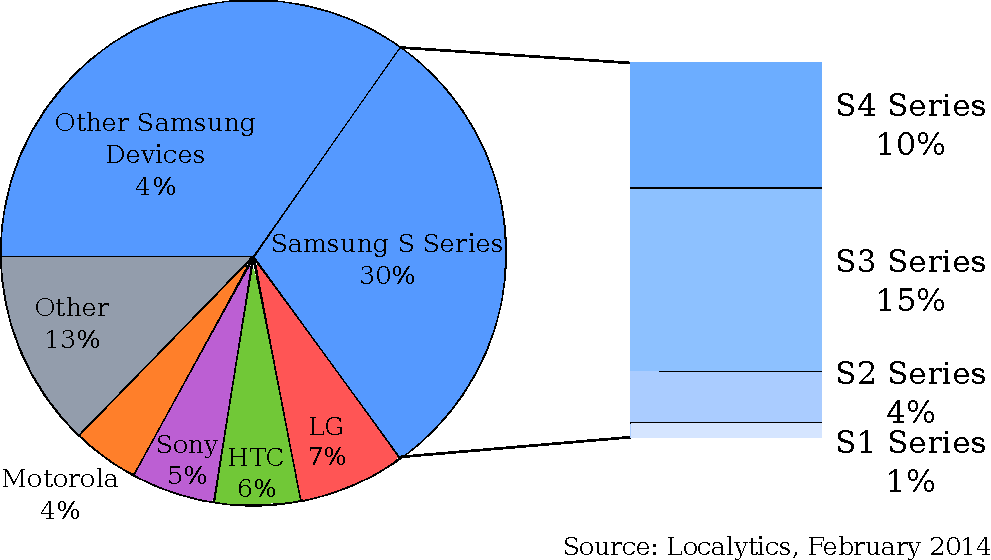
\includegraphics[width=0.75\textwidth]{android_market.pdf}
\caption{Global Android share~\citep{samsung_share_2014}. As this pie chart
illustrates, Samsung devices represent the 65\% of the Android worldwide market
share.}
\label{fig:android_market}
\end{figure}

According to the explanation of this section, in the following lines each 
experiment is described and evaluated. First, the default AdaptUIOnt reasoning 
performance comparing Pellet and \textit{Pellet4Android} is introduced in 
Section~\ref{sec:eval_default_ont}. Next, these reasoning engines are 
tested using a modification of the default ontology, increasing the ABox axioms 
set. This experiment is described in Section~\ref{sec:eval_abox}. 
Finally, the AdaptUIOnt default ontology's \ac{swrl} axioms set is increased to 
evaluate the performance of both reasoning engines when dealing with larger 
sets of rules (see Section~\ref{sec:eval_swrl}).


\subsubsection{Using the Default AdaptUIOnt Ontology}
\label{sec:eval_default_ont}

In this experiment the default version of the AdaptUIOnt ontology is used as 
input of the reasoning engines in order to evaluate their performance. As 
AdaptUIOnt has been designed to be a light ontology to be available to be used 
with mobile reasoning engines, this experiment shows how \textit{Pellet4Android} 
performs in comparison with the the results obtained by Pellet in a desktop 
environment. These results are shown in Table~\ref{tbl:eval_default_ont}.

\begin{table}
 \caption{Pellet and \textit{Pellet4Android} comparison loading the default 
AdaptUIOnt ontology.}
 \label{tbl:eval_default_ont}
 \footnotesize
 \centering
  \begin{tabular}{l l r r r r r r}
  \hline 
  &  & \multicolumn{2}{c}{\textbf{Axioms}} & 
  \multicolumn{3}{c}{\textbf{Results}}	\\
  \textbf{Device} & \textbf{Triples}& \textbf{ABox} & \textbf{\ac{swrl}}
  & \textbf{Mean} & \textbf{Median} & \textbf{Deviation}	\\
  \hline 
  Acer laptop	& 2,779	& 37  & 13 & 0.946 & 0.951 & 0.017	\\
  (Pellet)							\\
  Galaxy SIII Mini& 2,779& 37 & 13 & 2.764 & 2.737 & 0.127	\\
  (\textit{Pellet4Android})					\\
  Galaxy SIII	& 2,779	& 37  & 13 & 1.649 & 1.652 & 0.076	\\
  (\textit{Pellet4Android})					\\
  Nexus 10	& 2,779	& 37  & 13 & 5.147 & 5.122 & 0.205	\\
  (\textit{Pellet4Android})					\\
  \hline
\end{tabular}
\end{table}

Figure~\ref{fig:pellet_default} illustrates the differences of using Pellet or
\textit{Pellet4Android} when loading the default ABox and \ac{swrl} axiom sets in 
AdaptUIOnt. As is shown in Figure~\ref{fig:pellet_default} and in 
Table~\ref{tbl:eval_default_ont}, the performance of Pellet for Java 
environments is better in any case if we compare it with the Android based 
version. However, and although there are several differences depending on the 
used mobile device, the differences are small. This is specially remarkable in 
the case of the Samsung Galaxy SIII. This device performs a remarkable 1.649 
seconds, which is just approximately 0.7 slower than Pellet for Java.

\begin{figure}
\centering
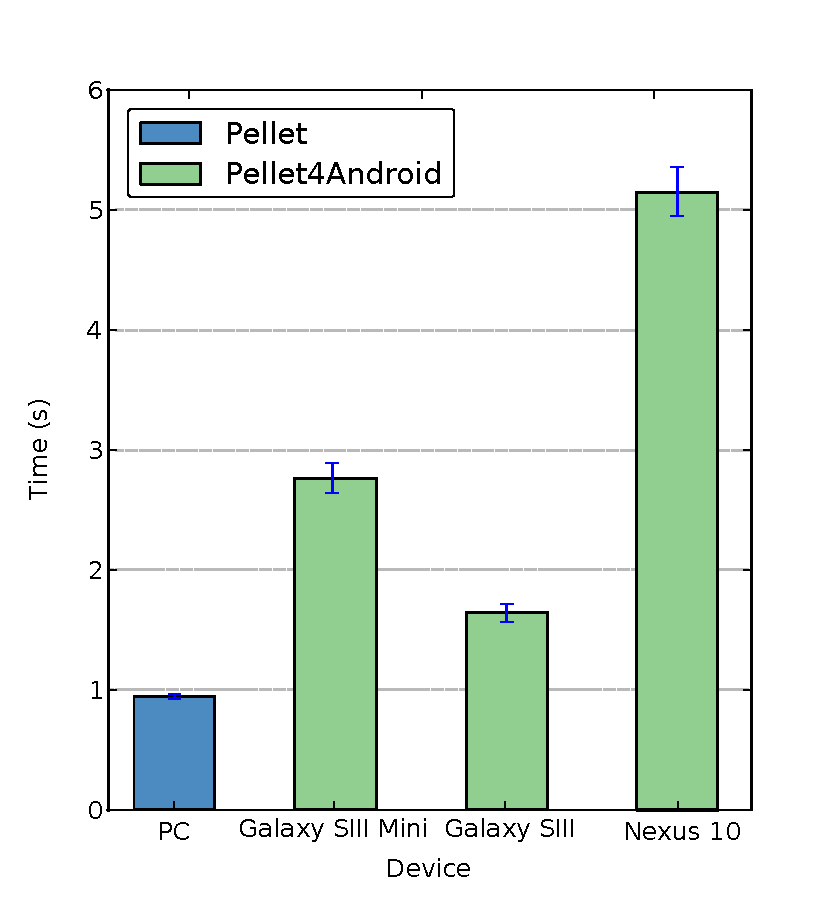
\includegraphics[width=0.75\textwidth]{pellet_default.pdf}
\caption{Pellet and \textit{Pellet4Android} performance comparison using the
default AdaptUIOnt ontology.}
\label{fig:pellet_default}
\end{figure}

\subsubsection{Incrementing the ABox Axioms Set}
\label{sec:eval_abox}

In this case the experiment consists in incrementing the ABox axioms set of 
the AdaptUIOnt ontology. As stated before, the ABox describes the attributes of 
instances, the roles between instances, and other assertions about instances 
regarding their class membership with the TBox concepts~\citep{abox_tbox}. 
The modification of the ABox has been carried out by incrementing the amount of 
instances in 5,000, 10,000, 15,000 and finally reaching 20,000 instances. Thus, 
with this experiment we want to evaluate how increasing the number of 
individuals might result into a performance penalization, specially in the case 
of \textit{Pellet4Android}. Table~\ref{tbl:eval_abox} shows the results of this
experiment.

\begin{table}
 \caption{Pellet and \textit{Pellet4Android} comparison loading the AdaptUIOnt 
ontology with an increment in the ABox axiom set.}
 \label{tbl:eval_abox}
 \footnotesize
 \centering
  \begin{tabular}{l l r r r r r r}
  \hline 
  &  & \multicolumn{2}{c}{\textbf{Axioms}} & 
  \multicolumn{3}{c}{\textbf{Results}}	\\
  \textbf{Device} & \textbf{Triples}& \textbf{ABox} & \textbf{\ac{swrl}}
  & \textbf{Mean} & \textbf{Median} & \textbf{Deviation}	\\
  \hline 
  Acer laptop & 12,779 & 5,000  & 13 & 3.014 & 3.012 & 0.034	\\  
  (Pellet)    & 22,779 & 10,000 & 13 & 3.903 & 3.905 & 0.052	\\
	      & 32,779 & 15,000	& 13 & 4.228 & 4.231 & 0.036	\\
	      & 42,779 & 20,000 & 13 & 4.539 & 4.541 & 0.042	\\
  \hline	      
  Galaxy SIII Mini& 12,779& 5,000& 13& 59.412& 59.508& 0.708	\\
  (\textit{Pellet4Android}) & 22,779 & 10,000 & 13 & 30.321 & 30.327 & 0.347 \\
	      & 32,779 & 15,000	& 13 & 87.957 & 87.018 & 1.108 	\\
	      & 42,779 & 20,000	& 13 & 183.882&183.879 & 2.101	\\
  \hline	      
  Galaxy SIII & 12,779 & 5,000	& 13 & 36.336 & 36.194 & 0.668	\\
(\textit{Pellet4Android})& 22,779 & 10,000 & 13	& 16.471 & 16.439 & 0.288\\
		& 32,779 & 15,000 & 13 & 45.387	& 45.593 & 0.729\\
		& 42,779 & 20,000 & 13 & 97.151	& 97.440 & 1.120\\
  \hline		
  Nexus 10	& 12,779 & 5,000  & 13 & 14.171 & 14.428 & 0.525\\
(\textit{Pellet4Android})& 22,779 & 10,000 & 13 & 9.024 & 9.065 & 0.291\\
		& 32,779 & 15,000 & 13 & 17.944& 17.969  & 0.496\\
		& 42,779 & 20,000 & 13 & 32.070	& 32.019 & 0.588\\
  \hline
\end{tabular}
\end{table}

Figure~\ref{fig:pellet_abox} illustrates the differences between Pellet and
\textit{Pellet4Android} when loading the AdaptUIOnt ontology with an increment 
applied to the ABox axioms set. As is shown in the chart (accordingly with
Table~\ref{tbl:eval_abox}) the performance of Pellet for Java environments 
keeps being better in comparison with the Android based version. While Pellet
maintains its performance under 5 seconds, Android devices require much more
time to perform the same reasoning. In fact, specially the Samsung Galaxy SIII 
Mini mobile device requires more than 180 seconds to evaluate the corresponding
20,000 instances, while the Samsung Galaxy SIII needs approximately 97 seconds 
and the Nexus 10 not more than 32.

\begin{figure}
\centering
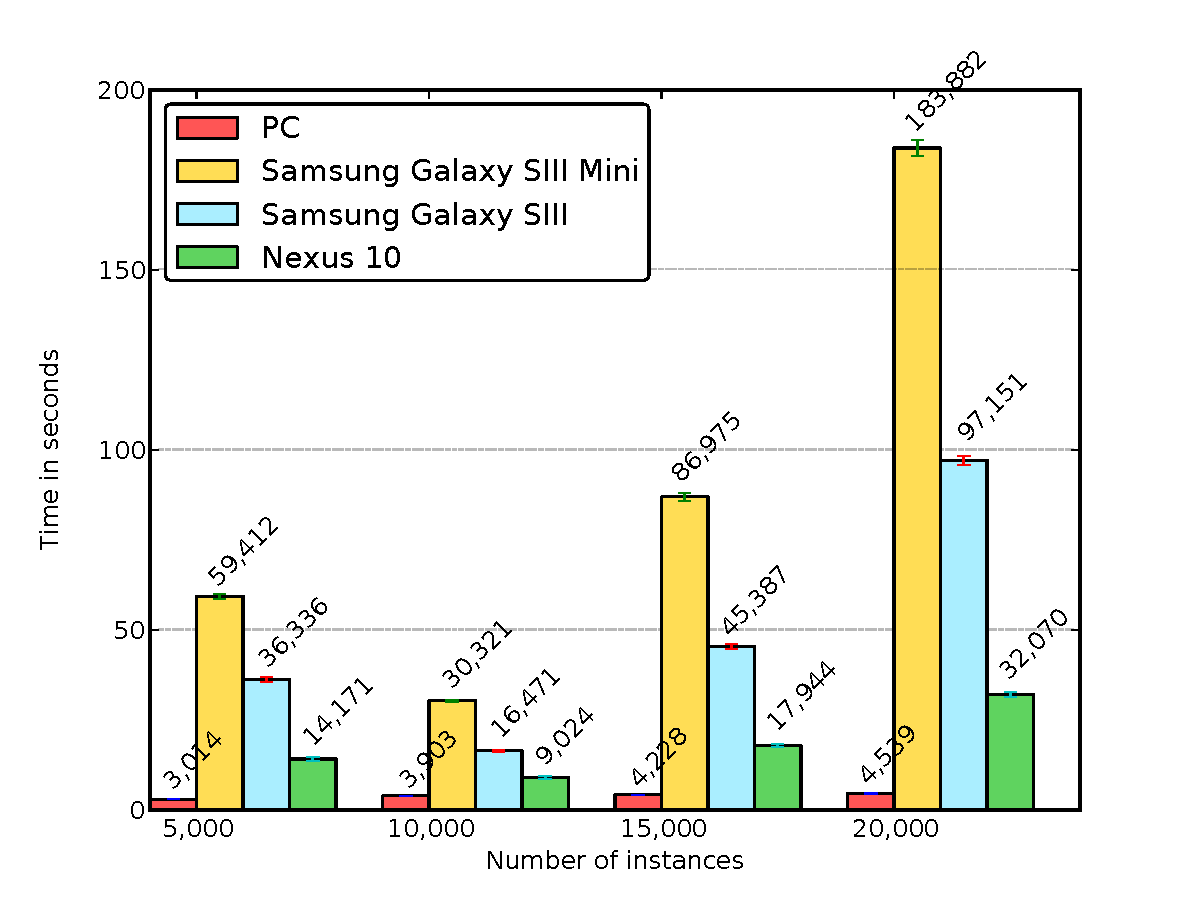
\includegraphics[width=0.95\textwidth]{pellet_abox.pdf}
\caption{Pellet and \textit{Pellet4Android} performance comparison using the
AdaptUIOnt ontology increasing the ABox axioms set.}
\label{fig:pellet_abox}
\end{figure}

\subsubsection{Incrementing the \ac{swrl} Axioms Set}
\label{sec:eval_swrl}

Finally, this last experiment consists in incrementing the \ac{swrl} axioms set of 
the AdaptUIOnt ontology, which collects the axioms related to the rules
included in the ontology. Using an amount of 5,000, 10,000, 15,000 and 
finally 20,000 rules we aim to evaluate how increasing the number of rules 
penalize the performance of Pellet, specially in the case of 
\textit{Pellet4Android}. Table~\ref{tbl:eval_swrl} shows the results of this
experiment.

\begin{table}
 \caption{Pellet and \textit{Pellet4Android} comparison loading the AdaptUIOnt 
ontology with an increment in the \ac{swrl} axiom set.}
 \label{tbl:eval_swrl}
 \footnotesize
 \centering
  \begin{tabular}{l l r r r r r r}
  \hline 
  &  & \multicolumn{2}{c}{\textbf{Axioms}} & 
  \multicolumn{3}{c}{\textbf{Results}}	\\
  \textbf{Device} & \textbf{Triples}& \textbf{ABox} & \textbf{\ac{swrl}}
  & \textbf{Mean} & \textbf{Median} & \textbf{Deviation}	\\
  \hline 
  Acer laptop & 82,779  & 37 & 5,013  & 4.770 & 4.732 & 0.141	\\
  (Pellet)    & 162,779 & 37 & 10,013 & 6.327 & 6.296 & 0.164 	\\
	      & 242,779	& 37 & 15,013 & 7.427 & 7.194 & 0.444 	\\
	      & 322,779	& 37 & 20,013 & 8.147 & 8.117 & 0.105	\\
  \hline
 Galaxy SIII Mini& 82,779 & 37 & 5,013  & 96.878  & 96.988  & 0.109 \\
(\textit{Pellet4Android}) & 162,779& 37 & 10,013 & 101.656 & 101.899 & 0.322 \\
	      & 242,779	& 37 & 15,013 & 243.981	& 244.011 & 0.298 \\
	      & 322,779	& 37 & 20,013 & 331.433	& 331.894 & 0.110 \\	
	\hline      
  Galaxy SIII & 82,779	& 37 & 5,013 & 84.121 & 84.121 & 0.869	\\
(\textit{Pellet4Android})& 162,779 & 37	& 10,013 & 74.248 & 74.103 & 0.250\\
		& 242,779 & 37 & 15,013	& 209.431 & 208.628 & 1.699 \\
		& 322,779 & 37 & 20,013	& 216.005 & 216.077 & 1.202 \\
\hline
  Nexus 10	& 82,779 & 37 & 5,013 & 22.317 & 22.471	& 0.333 \\
		& 162,779& 37 & 10,013& 45.193 & 44.736	& 1.312	\\
		& 242,779& 37 & 15,013& 85.543 & 88.134 & 5.490	\\
		& 322,779& 37 & 20,013& 107.151& 106.131& 2.749	\\
  \hline
\end{tabular}
\end{table}

Figure~\ref{fig:pellet_swrl} illustrates the differences between Pellet and
\textit{Pellet4Android} when running the different sets of \ac{swrl} axioms of the 
AdaptUIOnt ontology. As is shown in the chart it takes more time to evaluate the 
set of rules than the instances. In fact, the scale of the Y axis reaches 350 
seconds, while in Figure~\ref{fig:pellet_abox} the maximum mean reaches less 
than 200 seconds.

\begin{figure}
\centering
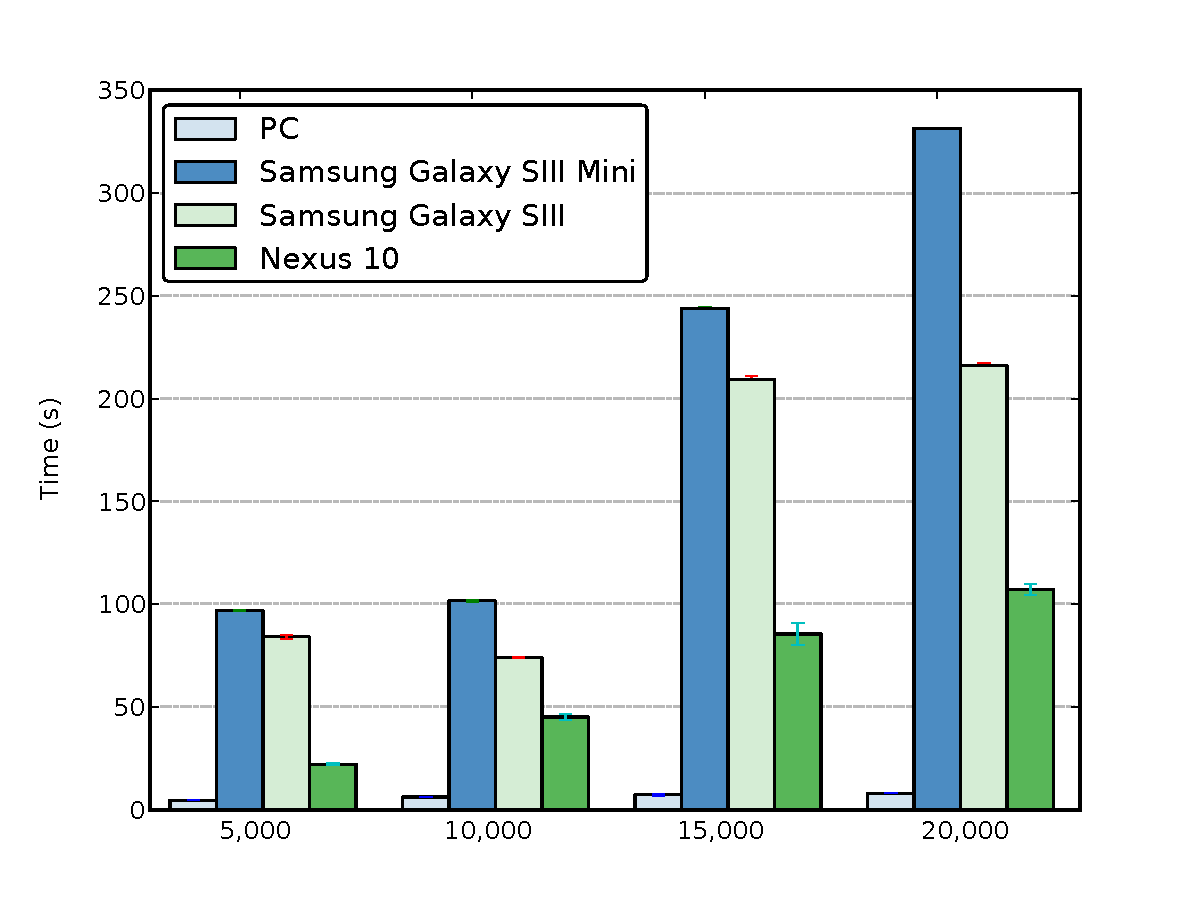
\includegraphics[width=0.95\textwidth]{pellet_swrl.pdf}
\caption{Pellet and \textit{Pellet4Android} performance comparison using the
AdaptUIOnt ontology increasing the \ac{swrl} axioms set.}
\label{fig:pellet_swrl}
\end{figure}

\subsubsection{Discussion}
\label{sec:performance_discussion}

During these experiments, and as is shown in Table~\ref{tbl:eval_default_ont}, 
Table~\ref{tbl:eval_abox} and Table~\ref{tbl:eval_swrl}, neither the TBox or 
RBox axioms sets have been modified. These collections belong to what is called 
the terminology knowledge in \ac{owl} 2, and it does not affect the performance of 
the reasoning process. Hence, the TBox and the RBox contain 266 and 22 axioms 
respectively during the experiments.

On the contrary, sets of 5,000, 10,000, 15,000 and 20,000 axioms have been added
to the ABox and \ac{swrl} axioms sets to demonstrate the performance penalization of 
when using large axioms sets with the tested reasoning engine. These 
modifications of the AdaptUIOnt ontology have been performed through several 
Python scripts, which have modified the corresponding default 
\textit{adaptui.owl} file.


\subsubsection{Conclusions}
\label{sec:performance_conclusions}

These results demonstrate that, although managing semantics in mobile devices is
possible, they still lack of more appropriate capabilities to perform reasoning
tasks. Nevertheless, \textit{Pellet4Android} is a good approximation of a 
reasoner to run on mobile devices. A native Pellet for Android port written in 
C++ would probably improve these results. But one of the AdaptUIOnt ontology's 
benefits is its lightness. Using less than 400 axioms, this ontology is able to 
model a full adaptation domain, remarking the user and his/her capabilities, the 
surrounding environment and the device characteristics. The results shown in 
Table~\ref{tbl:eval_default_ont} show how \textit{Pellet4Android} responses 
properly when dealing with the AdaptUIOnt ontology. However, more efforts in 
mobile reasoners would benefit these systems.

% Repasar bien
Regarding the ABox collection of axioms, the first conclusion that is extracted
from the results shown in Table~\ref{tbl:eval_abox} is that Pellet running in a 
PC has a very optimal response. For example, increasing the number of instances 
to almost 20,000 instances just reduces the response time in around 4 seconds 
(see Figure~\ref{fig:pellet_abox}). Increasing the ABox slows down the final 
performance, incrementing the number of seconds for loading the ontology. On 
the contrary, running this experiment in the mobile devices reveals a lack of 
efficiency. First, each device's hardware capabilities are taken into account. 
The first mobile device, the Samsung Galaxy SIII~Mini needs around 2.764 
seconds for loading the default AdaptUI ontology with its 37 ABox and 13 \ac{swrl} 
axioms. This same case takes 1.649 seconds in the Samsung Galaxy SIII and 5.147 
seconds in the Nexus 10. Although these figures might be appear to be enough 
considering we are dealing with limited Hardware, by increasing them in the 
same way that it has been done with the Acer laptop results into unmanageable
time responses. For instance, loading 5,032 ABox axioms takes 3.014 seconds for
the laptop and Pellet, for the Samsung Galaxy SIII Mini it takes 59.412 seconds,
36.336 seconds for the Samsung Galaxy SIII and 14.171 seconds for the Nexus 10. 

Nevertheless, these differences are more significant when dealing with the \ac{swrl}
axioms set. In this case, although Pellet's performance does not exceed 9 
seconds, the differences with the ABox axioms set are much bigger regarding
\textit{Pellet4Android}. In the best case, the Nexus 10 needs around 22 seconds
to reason over a 5,000 rules, while the Samsung Galaxy SIII Mini needs more 
than 90. This depicts the existing differences of performance depending on the
Android device we choose.
\subsection{Comparing AdaptUI with other \ac{aui} Solutions}
\label{sec:imhotep_comparison}

As a second part of the technical evaluation, in this section a comparison 
between AdaptUI and Imhotep is performed. The purpose of this section is to 
demonstrate that the capabilities of the AdaptUI platform improve the ones 
provided by the Imhotep framework. Hence, this section is organized as follows: 
First, in Section~\ref{sec:imhotep_vs_adaptui} the Imhotep framework and its 
main characteristics is introduced. Next, a use case using both adaptation 
platforms is detailed (see Section~\ref{sec:assisted_city_use_case}). Finally, 
in Section~\ref{sec:imhotep_discussion} and Section~\ref{sec:imhotep_conclusions} 
a discussion and several conclusions are presented.

\subsubsection{Imhotep}
\label{sec:imhotep_vs_adaptui}

Imhotep~\citep{almeida_imhotep_2011} is a framework developed and maintained at
the University of Deusto which aims to ease the development of adaptable and 
more accessible user interfaces. Designed by developers and for developers, this
framework allows to write their applications in a way in which they do not
have to worry about the adaptation of the user interface. This is possible 
through the definition of a series of preprocessor directives. These 
directives take into account both the user capabilities and the device 
characteristics. The developed applications are then uploaded to a public 
repository. Thus, the users can download them through an application download 
tool which sends to a server the user's and device's profile so the server 
compiles the best user interface for the current situation.

One of the benefits of Imhotep is the level of expression of the preprocessor
directives. Developers can establish their own variables and rules.
Listing~\ref{lst:imhotep_pseudocode} shows a piece of pseudo-code where the
developer defines new variables.

\inputminted[linenos=true, fontsize=\footnotesize, frame=lines]{java}{5_experiments_and_results/imhotep_pseudocode.txt}
\captionof{listing}{Imhotep pseudo-code defining variables~\citep{imhotep_website}.\label{lst:imhotep_pseudocode}}


These variables, rules and possible values are defined by the developer using a
web based wizard. Furthermore, the concepts, such as \textit{``resolution is 
big''}
are created by the system taking into account the information of the mobile
devices (provided by \ac{wurfl}~\citep{wurfl}) and pondering it with their popularity
(with Google Trends~\citep{trends} data).

In order to fully understand how Imhotep works, 
Figure~\ref{fig:imhotep_architecture}
illustrates its architecture design. As can be seen in the figure, Imhotep is
divided into 4 modules:

\begin{itemize}
    \item The first one is the Application Downloader, which is a tool installed
    in the user's device to connect to the repository and download adapted
    applications.
    
    \item The \ac{rest} server contains the application repository. Once a user 
    selects a desired application, the server will:
    
    \begin{itemize}
      \item Use the Fuzzy Knowledge-Eliciting Reasoner to infer new values with
      the user and device configuration and the variables and rules established
      by the developer of the application.
      
      \item Call the Preprocessor to select only the code that the final user
      requires.
      
      \item Delegate the compilation of the application to the Compiler Manager.
      Currently the \ac{rest} server only supports Android, but other compilers could
      be easily added.
      
      \item Store the compiled application in the Compilation Cache, so future
      requests will not require to pass through the whole process if they have
      the same configuration values.
    \end{itemize}
    
  \item The Wizard: developers use the wizard to establish the variables and the
  possible values of those variables. It uses the trends database to show the
  different values given a concrete user and a concrete device.
  
  \item The Capacity Tester. Users have to create a user profile with their
  capabilities. The Capacity Tester will gather those capabilities by testing
  them. The Current application is just a proof of concept of how the Capacity
  Tester should work.
\end{itemize}

\begin{figure}[H]
\centering
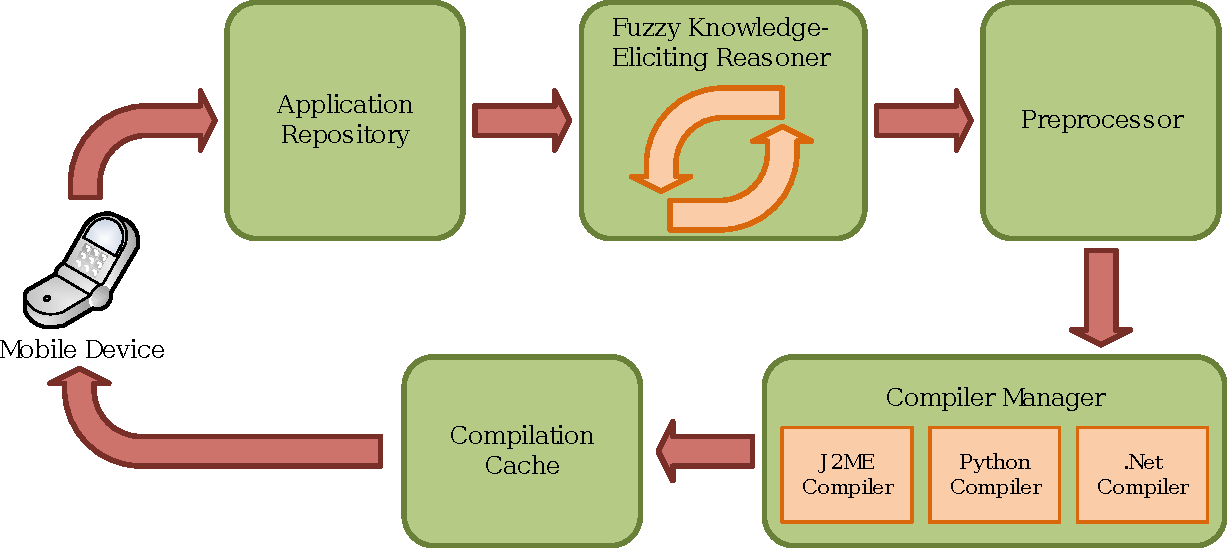
\includegraphics[width=0.90\textwidth]{imhotep_architecture.pdf}
\caption{The Imhotep architecture~\citep{imhotep_website}.}
\label{fig:imhotep_architecture}
\end{figure}

The preprocessor directives define how the final source code must be generated, 
providing conditions for certain regions of code to be added or skipped and 
adding the corresponding \ac{ui} variables that the preprocessor will adapt for each
compilation. The preprocessor identifies the directives when they start by //\#
in languages that support inline comments starting by //, such as Java, C\# or
C++, \#// in languages that support inline comments starting by \#, such as 
Python or Perl, and '// in VB.NET.

The preprocessor can avoid the compilation of fragments of code if certain 
conditions are met. These conditions can include calls to functions provided 
by the system. Basic string and \textit{math} functions are available, including
\textit{lowercase}, \textit{trim}, \textit{contains}, \textit{round} or 
\textit{sqrt}, as well as functions to check if a certain variable is 
available. The conditions can be embedded, as shown in the code below. The 
syntax of the conditions is  based on the syntax used by the Python programming 
language. The following code shows an example of using preprocessor directives 
in Java. During compiling time this code will be analysed by the framework 
taking into account the defined variables and their values. Therefore, the final 
binaries will contain just one reference to one of the methods shown in 
Listing~\ref{lst:preprocessor_directives}.


\inputminted[linenos=true, fontsize=\footnotesize, frame=lines]{python}{5_experiments_and_results/preprocessor_directives.py}
\captionof{listing}{Using the Imhotep framework through preprocessor 
directives~\citep{imhotep_website}.\label{lst:preprocessor_directives}}


Developers ask for user and device capabilities in these conditions. For 
example, one directive could state that if the user is blind the application 
should use a voice based interface. Five categories of user capabilities were 
defined (see Figure~\ref{fig:imhotep_user_capabilities}).


\begin{figure}[H]
\centering
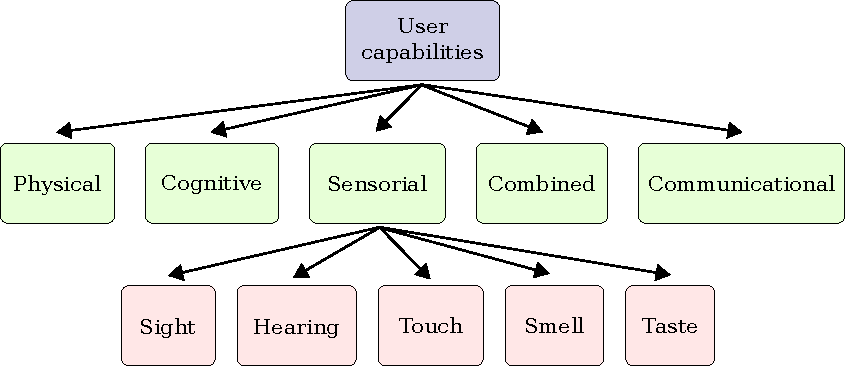
\includegraphics[width=0.90\textwidth]{imhotep_user_capabilities.pdf}
\caption{The set of Imhotep's user capabilities~\citep{imhotep_website}. As is
shown, user capabilities are classified into 5 different groups: physical, 
relative to user's motor skills; cognitive, which deals with memory and 
comprehension capabilities; sensorial, including capabilities related to 
sight, hearing, touch, smell and tast; combined, including combination of 
different disabilities; and communicational, which deals with speech.}
\label{fig:imhotep_user_capabilities}
\end{figure}

Now that the Imhotep framework has been introduced, a comparison between AdaptUI and
Imhotep running the same experiments is presented. Despite the fact that both solutions
have the same purpose (to help reducing the boundaries for those who cannot
properly interact with a user interface), their differences are substantial.
Imhotep directly depends on a server (allocated in the University of Deusto)
while AdaptUI runs 100\% in the mobile phone, performing the adaptation on the
fly. 

\subsubsection{Use Case: AssistedCity}
\label{sec:assisted_city_use_case}

As said before, Imhotep is a framework for developers which provides a 
preprocessor directive based procedure to build adaptive user interfaces. The 
Imhotep framework was originally tested with AssistedCity\footnote{\url{
https://github.com/aitoralmeida/imhotep/tree/master/PiramideRestServer/deploy/piramide/applications/AssistedCity/1.0.0.0/project}}. 
AssistedCity is a tour 
guide application which guides the user taking into account several points of interest 
categories (i.e., monuments, museums, restaurants, and so forth) that the user 
needs to choose from a menu. Then, using the camera and through an Augmented 
Reality interface the application guides the user to the desired point of 
interest. As a demonstrator of the Imhotep framework, this application was 
developed using several preprocessor directives which take into account sight 
sensory capabilities, hearing capabilities and device's screen size, to adapt 
the user interface of the application. Hence, we have chosen the same use case to 
evaluate the results of the adaptation using the corresponding platform.

This evaluation is split in two different parts. First, a visual comparison of
the resulting adaptations is shown. Then, we focus on the performance of both
solutions, specially on the required time to get the whole processes finished.

For the adaptation using Imhotep, an extra application is needed to send the 
user's and device's characteristics to the Imhotep server. 
Listing~\ref{lst:variables} shows the variables file used by Imhotep to perform
the corresponding adaptation. This file is completed by the user when he/she 
uses the cited application. Once the variables file is completed, the user is 
able to download the desired provided application from the Imhotep server.


\inputminted[linenos=true, fontsize=\footnotesize, frame=lines]{json}{5_experiments_and_results/variables.json}
\captionof{listing}{The variables file, in which device characteristics and user 
capabilities are described.\label{lst:variables}}


On the contrary, the corresponding AdaptUI models for the user and the device 
are represented  through the AdaptUIOnt ontology, and there is no need for 
external servers. The similar user and device situation is represented as 
follows, in Table~\ref{tbl:adaptui_repr}:

\begin{table}[H]
 \caption{User and device characteristics representation in AdaptUIOnt.}
 \label{tbl:adaptui_repr}
 \footnotesize
 \centering
\begin{tabular}{l l l l }
\hline 
\textbf{Entity} & \textbf{Class}   & \textbf{Data property}  & \textbf{value}\\
\hline
\textit{User}&
\textit{Display} & \textit{userDisplayBrightnessIsStatic}  &\textit{false}\\
\textit{(UserCharacteristics)}& & \textit{userDisplayIsApplicable} 	   
&\textit{false}\\
&\textit{Audio} & \textit{userDisplayApplicableIsStatic}   &\textit{false}\\
&		 & \textit{userAudioHasApplicable} 	   &\textit{true} \\
&		 & \textit{userAudioApplicableIsStatic}    &\textit{false}\\
&		 & \textit{userAudioHasVolume}  	   & $5$ 	  \\
&\textit{Interface}& \textit{userInterfaceInput} 	   &\textit{haptic}\\
&		 & \textit{userInterfaceOutput} 	   &\textit{default}\\
&\textit{Experience}& \textit{userHasExperience} 	   &\textit{high} \\
&\textit{View}	 & \textit{userViewIsStatic}		   &\textit{false}\\
&\textit{Other} 	 & \textit{userHasLanguage}		   
&\textit{English}\\
		 & \textit{vibration} 			   &\textit{true}\\
\hline
\textit{Device} & \textit{DeviceScreenResolution} & 
\textit{deviceHasScreenResolution} & $1280 x 720$\\
\textit{(DeviceCharacteristics)} & \textit{OS} & \textit{deviceHasOSVersion} & 
$4.3$\\
\hline
\end{tabular}
\end{table}


The results of the adaptations are illustrated in the following figures. First,
Figure~\ref{fig:ac_default} shows the default user interface for the main menus 
of the application. It originally consists of several visual icons representing 
different venues categories (i.e., bars, restaurants, cafés, and so on). Once the 
user chooses one option, a list with the nearer corresponding type of venues
is presented.

\begin{figure}[H]
\centering
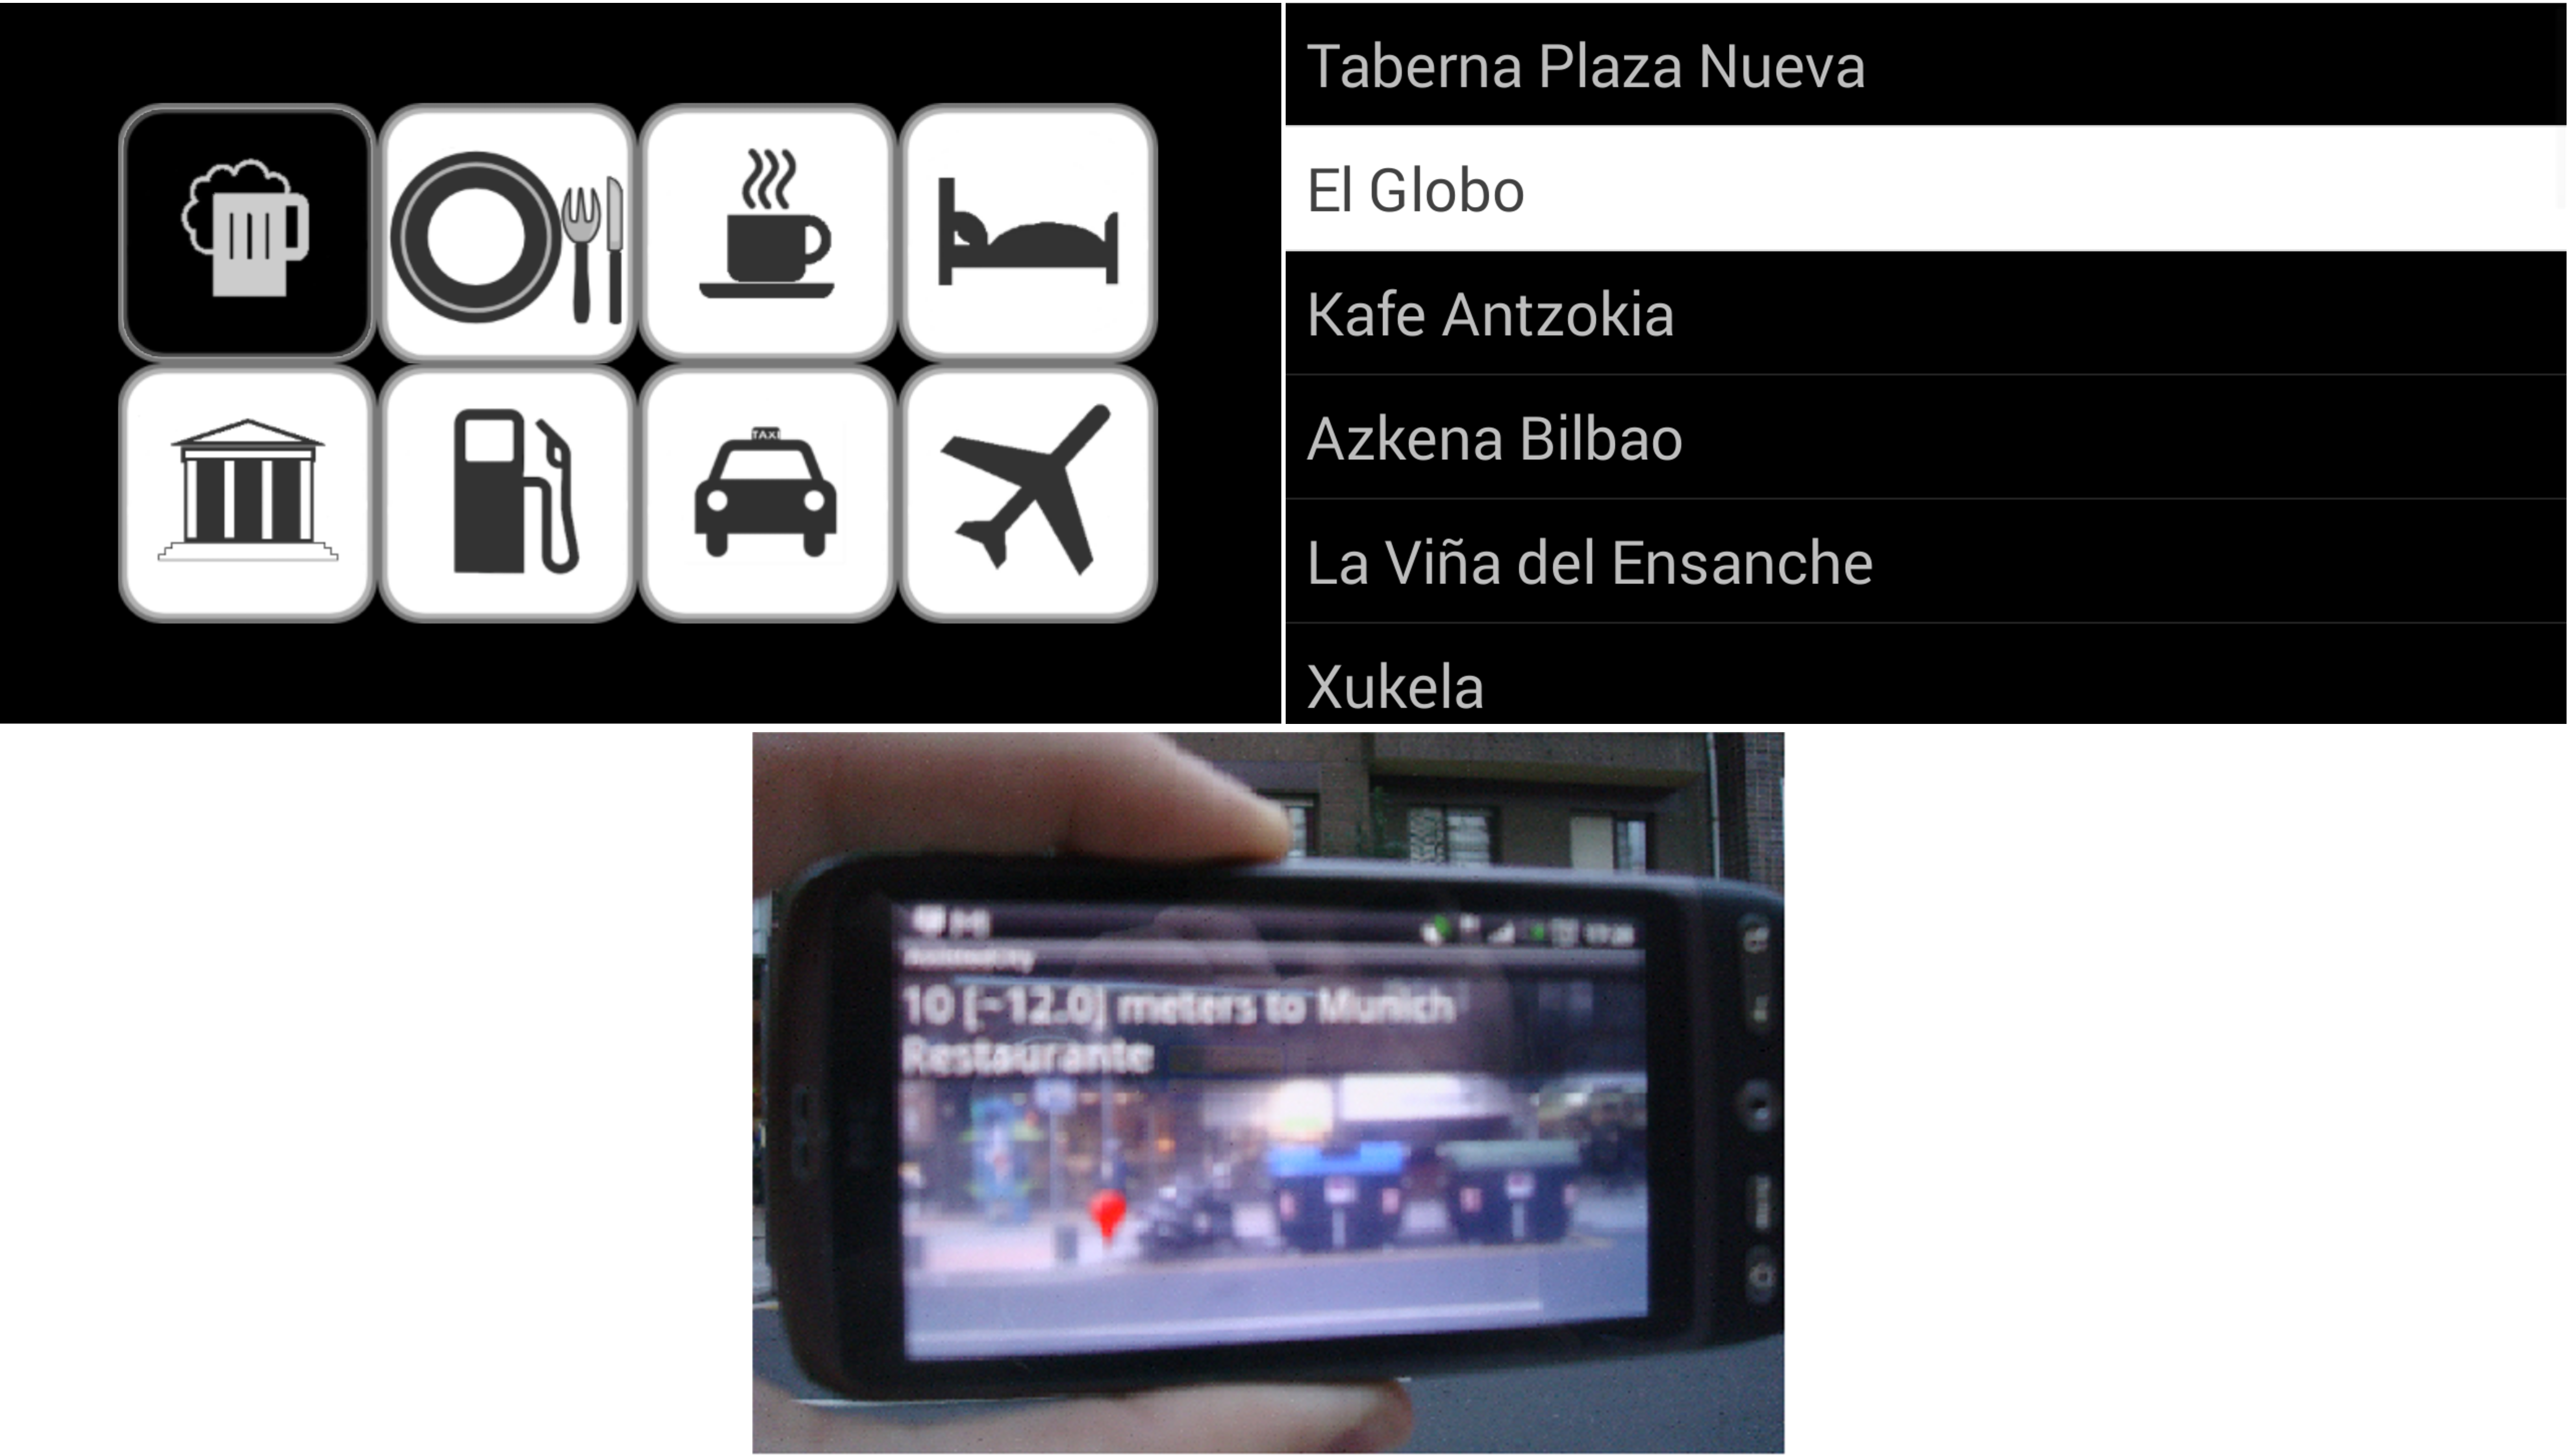
\includegraphics[width=0.75\textwidth]{ac_default.pdf}
\caption{AssistedCity default menus and user interface.}
\label{fig:ac_default}
\end{figure}

Next, a comparison between the two adaptations is illustrated through 
Figure~\ref{fig:ac_adapted}. On the left the adaptation performed by Imhotep is 
shown. The parameters detailed in Listing~\ref{lst:variables} for the user and 
device characteristics are sent to the Imhotep server. Then, the corresponding
application is generated and send back to the user. On the contrary, on the 
right side of Figure~\ref{fig:ac_adapted} there is the adaptation performed by 
AdaptUI. Considering the input detailed in Table~\ref{tbl:adaptui_repr} AdaptUI 
performs the corresponding adaptation (depending on the set of specified rules).
The adaptation performed by AdaptUI matches the input capabilities shown in
Table~\ref{tbl:adaptui_repr}, which represents better the user capabilities
than the specification given by Listing~\ref{lst:variables}.

\begin{figure}[H]
\centering
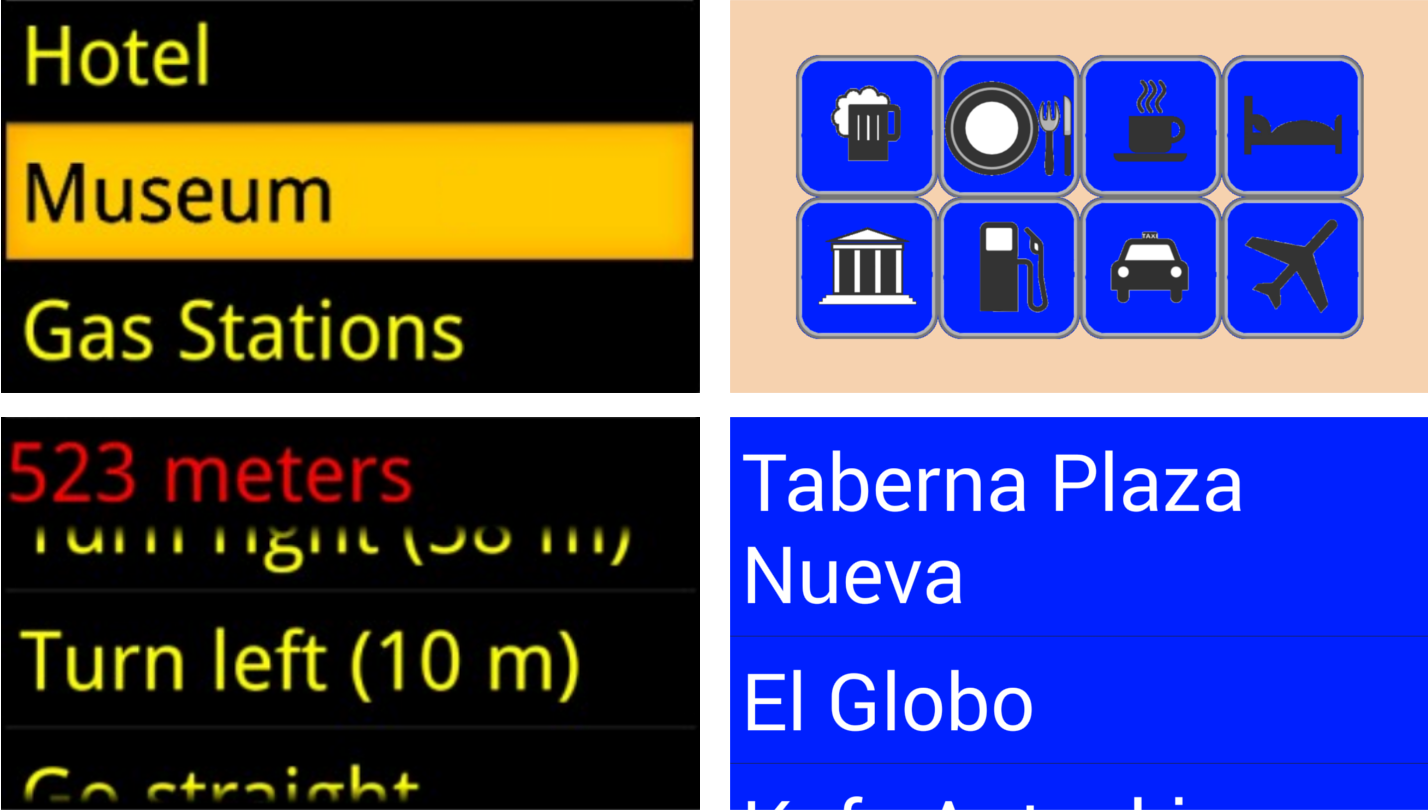
\includegraphics[width=0.60\textwidth]{ac_adapted.png}
\caption{AssistedCity adapted by Imhotep (left) and AdaptUI (right) taking 
into account the corresponding inputs shown in Listing~\ref{lst:variables} and 
Table~\ref{tbl:adaptui_repr}.}
\label{fig:ac_adapted}
\end{figure}


% the difference adaptation for the main menu of 
% the AssistedCity application. On the left, there is the adaptation performed by
% Imhotep using the parameters detailed in Listing~\ref{lst:variables} for the 
% user and device characteristics.

Regarding the time performance evaluation in Table~\ref{tbl:imhotep_timing}, it 
shows the time required by Imhotep to adapt AssistedCity. As seen through this 
table, if the server maintains a cache of the already adapted applications for 
the specific user and device the response of the system does not exceed 1.3
seconds. 

\begin{table}[H]
 \caption{Imhotep framework time analysis. The figures under Mean, Median and
 standard deviation (Std. deviation) are represented in seconds.}
 \label{tbl:imhotep_timing}
 \footnotesize
 \centering
\begin{tabular}{l l l l l l l}
%  S[round-precision=2]
  \hline 
  \textbf{Device} & \multicolumn{3}{c}{\textbf{Cached 
  data}} & \multicolumn{3}{c}{\textbf{Non cached data}}\\
  & \textbf{Mean} & \textbf{Median} & \textbf{Deviation} &  \textbf{Mean} 
  & \textbf{Median} & \textbf{Deviation}\\
  \hline    
  Galaxy SIII~Mini & $1,257$ & $1,237$ & $0,247$ & $15,125$ & $15,034$ & 
$0,445$ \\
%   
  Galaxy SIII & $1,175$ & $1,107$ & $0,239$ & $15,094$ & $14,950$ & $0,501$ \\
%   
  Nexus 10 & $1,211$ & $1,184$ & $0,180$ & $15,115$ & $15,033$ & $0,492$ \\
 \hline
\end{tabular}
\end{table}

On the contrary, AdaptUI does not require an external server, and it does not 
use any cache. Thus, the required time for the adaptation depends mostly on the 
hardware of the device running the reasoning process. Table~\ref{tbl:imhotep_vs_adaptui}
compares the means of using Imhotep or AdaptUI for an adaptation. In the case of 
AdaptUI, a light change in context triggers the process. Obviously, this represents
one of the most significant benefits of AdaptUI, as the platform is able to 
dynamically react to these changes. On the contrary, a user of AssistedCity will
need to indicate the new situation in the variables file, and the reasoning process
will start again in the Imhotep server.

\begin{table}[H]
 \caption{Comparing Imhotep and AdaptUI time performance. The mean is 
represented in seconds.}
 \label{tbl:imhotep_vs_adaptui}
 \footnotesize
 \centering
\begin{tabular}{l l l l}
  \hline 
  \textbf{System} & \textbf{Platform} & \textbf{Cache/Trigger} & \textbf{Mean}\\
  \hline
  Imhotep 	& Galaxy SIII~Mini	& Cached		& $1.257$\\
		&  			& Not cached		& $15.125$\\
		& Galaxy SIII 		& Cached		& $1.211$\\
		&  			& Not cached		& $15.115$\\
		& Nexus 10 		& Cached		& $1.175$\\
		&  			& Not cached		& $15.094$\\
  \hline
  AdaptUI 	& Galaxy SIII~Mini	& Context change	& $1.899$\\
		& Galaxy SIII		& Context change	& $1.544$\\
 		& Nexus 10 		& Context change	& $1.213$\\
  \hline
\end{tabular}
\end{table}

\subsubsection{Discussion}
\label{sec:imhotep_discussion}

Imhotep was conceived in 2010, when the hardware characteristics of the available 
Android devices was still limited. First 1 \ac{ghz} processors started to power 
these devices, and their \ac{ram} memory vaguely exceeded 500 \ac{mb}. Considering 
these limitations, Imhotep was designed following the same approach that several 
solutions cited in Chapter~\ref{cha:state_of_the_art} used: externalizing the 
computational complex processes to an external server. Hence, in Imhotep the 
developers have to use several available preprocessor directives where the user 
interface alternative code has to be included. Then, their source code is 
uploaded to an external server, which would generate the corresponding binaries 
(according to user's requests) with the corresponding adaptation. These requests 
include the characteristics of the mobile device and the user's profile. 

Although Imhotep was a good approximation as a tool for developers to write 
applications with adaptive user interfaces, we have found several problems
in it:

\begin{itemize}
  \item Regarding final users, \textit{Imhotep requires an extra tool for 
  downloading the required application} with the corresponding and adapted user 
  interface. This means that every time the user requires a different adaptation 
  the profile configuration process is launched. Thus, if there is no cached data 
  in the server, it will cause a significant delay in the adaptation process.
  
  \item Besides, \textit{Imhotep depends on Internet connection} for for the 
  adaptation, which might be problematic. As an external server is needed to 
  perform the adaptive operations and source code compiling, there is the 
  possibility of a server or network failure, which would obviously affect or 
  even cancel the whole process.
  
  \item \textit{Context is not taken into account for the adaptation}. Only the 
  user and the characteristics of the current device were considered. Several 
  examples of the benefits of including context for the adaptation process have
  been presented during this section.
\end{itemize}

On the contrary, AdaptUI was conceived during 2013, when multi-core kernels and
CPUs were already deployed into mobile devices. These new characteristics 
increased their capabilities, making possible more complex processing. 
Therefore, AdaptUI first designs were definitely based on Android. This brings 
the whole adaptation process to the mobile. This means that, on the one hand, 
there is the advantage of not depending on the network or an external server to 
process anything. But it also means that the workload has to be managed by a 
hardware not as powerful or capable as a computer's one. As also detailed in 
Table~\ref{tbl:imhotep_vs_adaptui}, the adaptation performance relies on the
each device's hardware capabilities. 

Besides, AdaptUI includes the current context situation in the equation for the 
user interface adaptation. This fact presents several challenges and possibilities, 
as is considered in AdaptUI as a trigger for different situations involving the 
user and the device.


\subsubsection{Conclusions}
\label{sec:imhotep_conclusions}

During this section a comparison between AdaptUI and Imhotep has been performed.
Imhotep is a framework for easing the adaptation of user interfaces. In the 
presented figures and tables both solutions evaluation has been illustrated. 
The resulting adapted interfaces and the corresponding performance of both 
platforms have been shown. Next, we summarize our experiences through this 
evaluation with several considerations in the following lines.

As Imhotep needs an external server for the complex processing of the user 
interface adaptations, maintaining a cache is vital for this system. On the 
contrary, and as shown in Table~\ref{tbl:imhotep_timing}, the response time 
from rebuilding the whole source code results in a 15 seconds delay. Comparing with
the cached results, which imply less than 1.5 seconds to perform the same 
operation is clear that the difference is significant. Nevertheless, one of the 
benefits of this solution is that, as the adaptation process is delegated to an 
external server, is not important which device is being used by the user. The
current device has just to be compatible with the applications available in the
server.

One of the main problems of Imhotep is that context is not taken into account 
for the adaptations. The explanation for this decision was based on the time 
limitation of Imhotep for performing a complete adaptation. 
Figure~\ref{fig:imhotep_comparison} illustrates how operating without cached 
data takes around 15 seconds for receiving the corresponding user interface in 
the device. This means that the context might change during this period of time. 
On the other side, the cache was conceived to store information about the 
profile of the user and the device that might not change during time. By using 
this cache the adaptations were sent back to the device in less than 2 seconds.

\begin{figure}[H]
\centering
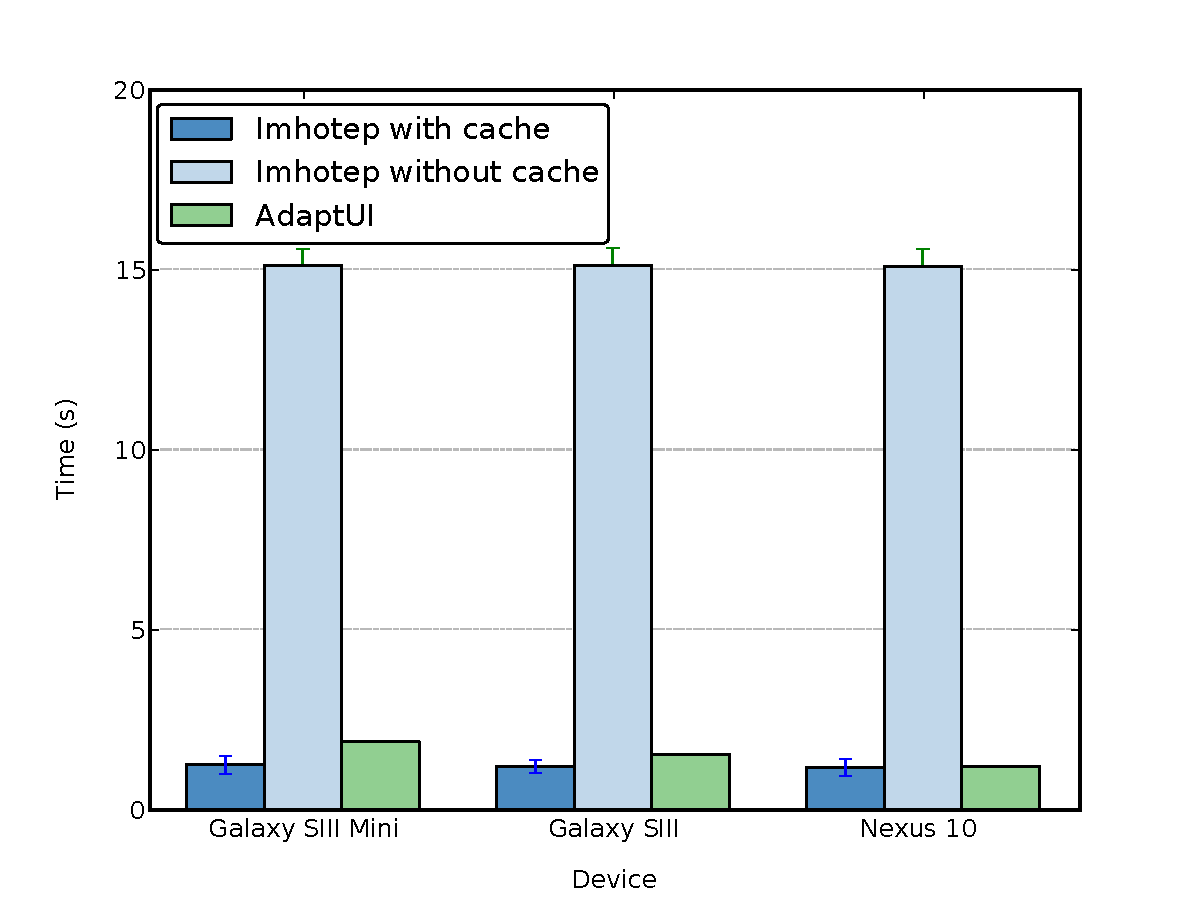
\includegraphics[width=0.75\textwidth]{imhotep_comparison.pdf}
\caption{Receiving the corresponding adapted user interface for different
devices using Imhotep without cache.}
\label{fig:imhotep_comparison}
\end{figure}


Imhotep time responses are obtained as the result of the addition of three
different processes. The first one is the required time in terms of networking,
that takes to send the adaptation request from the device to the adaptation 
server. Secondly, the required time to process the request, compile and generate 
the adapted version (around 14 seconds). And finally, the time needed to send 
the adaptation back to the user's device with the corresponding user interface. 

On the other hand, AdaptUI performance does not depend on the network traffic, 
as it runs 100\% in the mobile device. Thus, the obtained performance results 
depend only on the hardware and software capabilities of the device. The 
triggers are launched by the user for Imhotep and by a context change for 
AdaptUI respectively. This is shown in Table~\ref{tbl:imhotep_vs_adaptui}.

Regarding the presented arguments, we conclude that:

\begin{enumerate}[label=\alph*]
  \item Imhotep's performance when using a cache is similar (even better) when
  network conditions are optimal. 
  
  \item As Imhotep does not carry out complex operations in the mobile devices,
  leaving this workload to an external server, the hardware specifications of 
  the current device are not as important as in AdaptUI.
  
  \item On the contrary, this dependency carries several drawbacks. For 
  example, a network failure would leave the adaptation process incomplete.
  
  \item Besides, although working with a cache results in similar time responses
  than AdaptUI, first adaptations of each application will cost a high time to
  be performed. During this time (around 15 seconds under normal circumstances)
  the context of the user might change, and it is possible for the user to 
  reject the adaptation.
  
  \item As AdaptUI takes the context into account, the adapted solutions are
  more characterized for the current user situation.
  
  \item Although depending on the device's hardware, it might result into slower
  adaptations, managing small semantic models (as AdaptUIOnt) is still 
  manipulable by the platform. Besides, as the smartphones market grows in terms
  of hardware capabilities, the performance of such systems will be increased.
  
  \item AdaptUI does not consider explicit physiological user capabilities. On 
  the contrary, Imhotep works with a user model in which it is necessary to
  provide several physiological based capabilities. This results into a non
  practical solution, as we lack of medical knowledge.
  
  \item Another benefit from AdaptUI is the automation of the adaptation 
  through several sets of adaptation rules. These rules, not considering 
  explicit physiological user capabilities, infer knowledge about the user that
  is vital for the adaptation. The whole set of rules that manages the adaptation
  process in AdaptUI are detailed in Section~\ref{sec:adaptui_rules}.
\end{enumerate}
\subsection{Scenarios}
\label{sec:scenarios}

In the previous section several quantitative experiments have been presented.
The experiments have illustrated the performance differences considering the 
required time to manage the AdaptUIOnt ontology and Imhotep. Regarding the 
ontology itself, AdaptUI takes into account many context situations, user's 
capabilities and device's characteristics. This makes difficult to evaluate 
every one of these settings in real environments. In this section, several 
hypothetical scenarios are presented simulating the behaviour of the analysed 
adaptive systems in more complex situations.

The scenarios are included in the evaluation of AdaptUI compared to Imhotep.
Consequently, both adaptation processes are taken into account for the 
resulting adaptation and the presented scenario conditions. Hence, the scenarios
represent three stereotypical situations which might require a user interface 
adaptation:

\begin{itemize}
  \item First, in the first scenario the situation is characterized by several
  context parameters that limit certain user capabilities. Consequently, 
  AdaptUI would have to consider the user as an updated version of 
  himself/herself, taking into account the new set of capabilities that 
  he/she has due to the context situation.
  
  \item In the second scenario, a situation in which the user capabilities are 
  delimited by a set of tasks that form an activity is presented. The user is 
  impeded to act normally. Therefore, the AdaptUI platform would have to be 
  aware of this limitation. 
  
  \item The last scenario simulates a situation where the user suffers from a 
  certain disability, so the platform should adapt the user interface 
  accordingly.
\end{itemize}

Each scenario is presented as follows:

\begin{itemize}
  \item First, an introduction to the problem to be evaluated is described.
  
  \item Secondly, the scenario situation is presented. It is also summarized with
  a table indicating the main characteristics of the three main entities.
  
  \item Thirdly, the adaptation process by Imhotep and AdaptUI is detailed.
  
  \item Finally, each scenario presents several conclusions after a brief 
  discussion.
\end{itemize}

\subsubsection{Scenario 1: Limitations Caused by Context Conditions}
\label{sec:scenario1}

This scenario introduces several limitations that context might induce to 
certain user capabilities. As context is considered as a significant entity in 
AdaptUI, this scenario aims to solve a situation in which it impedes the user to
interact properly. On the contrary, Imhotep does not include the context 
situation for adapting the user interface. Thus, it would not be possible to 
have a coherent result regarding the proposed scenario. The following 
lines introduce the cited scenario:

John is going home after work. He lives and works in Rovaniemi, one of the
northernmost and coldest regions in Finland. As can be seen in 
Table~\ref{tbl:scenario1}, John does not suffer from any disability. He removes
his gloves and then he proceeds to send a \ac{sms} to his wife. The current 
temperature is $-10$~ºC.

\begin{table}
 \caption{Scenario 1 situation summary.}
 \label{tbl:scenario1}
 \footnotesize
 \centering
\begin{tabular}{l l}
  \hline 
				& \textbf{Scenario 1} 		\\
  \hline
  User \\
  \qquad - Personal data 	& John, $36$ years old, Finnish 	\\
  \qquad - Activity	 	& Sending a \ac{sms}		 	\\
  \qquad - Known disabilities 	& None			 	\\
%   \hline
  Context \\
  \qquad - Location 		& Relative: Rovaniemi, Finland	\\
				& Absolute: $66.497109$, $25.724977$\\
  \qquad - Time			& $18$:$35$				\\
  \qquad - Brightness		& $600$ \ac{lx}			\\
  \qquad - Temperature		& $-10$ ºC			\\
%   \hline
  Device 			& Samsung Galaxy SIII		\\
				& Battery: $85$\%			\\
  \hline
\end{tabular}
\end{table}

AdaptUI covers this situation through the following steps. First, the platform
considers through the user model that John does not suffer from any 
disabilities. Analysed by the Capabilities Collector, AdaptUI does not find 
disabilities that would limit future adaptations. 
Table~\ref{tbl:user_profile_scenario1} shows the semantic representation of the 
model, carried out by the Semantic Modeller, that fits John’s profile. 

\begin{table}
 \caption{User profile for Scenario 1.}
 \label{tbl:user_profile_scenario1}
 \footnotesize
 \centering
\begin{tabular}{l l l }
  \hline 
  \textbf{Class}  & \multicolumn{2}{c}{\textbf{Scenario 1}}		\\
		  & \textbf{Data property} & \textbf{value} 		\\
  \hline
  \textit{Display}& \textit{userDisplayBrightnessIsStatic*} & true	\\
		  & \textit{userDisplayIsApplicable}	    & true	\\
  \textit{Audio}  & \textit{userDisplayApplicableIsStatic}  & false	\\
		  & \textit{userAudioHasApplicable} 	    & true 	\\
		  & \textit{userAudioApplicableIsStatic}    & false 	\\
		  & \textit{userAudioHasVolume}  	    & $4$ 	\\
  \textit{Interface}& \textit{userInterfaceInput}	    & haptic	\\
		  & \textit{userInterfaceOutput} 	    & default	\\
  \textit{Experience}& \textit{userHasExperience} 	    & high	\\
  \textit{View}	  & \textit{userViewIsStatic}		    & false	\\
  \textit{Other}  & \textit{userHasLanguage}		    & Finnish	\\
		  & \textit{vibration} 			    & true 	\\
  \hline
\end{tabular}
\end{table}

Regarding John’s model, it can be seen how it is configured as an open model for
future adaptations. Besides, most of the preferences are configured as default. 
The only property that is limited from the model is the brightness, which John
has established as a static property. This means that AdaptUI understands that
this property should not be adapted no matter what the context situation is.
As the contrast and the volume are not static, the modelled integer values are
considered as preference values and not a limitation for the rules. This means
that John prefers a volume level of 4, but he allows the system to manage it if
certain conditions are met. These integer values are different depending on the
used platform. In this case, as these experiments run over the Android platform,
they refer to Android values \citep{android_volume}. 

Table~\ref{tbl:user_profile_scenario1} shows the semantic representation of 
this model which fits John’s profile, using the AdaptUI ontology detailed in 
Chapter~\ref{cha:ontology_model}. The asterisk marks a property that is marked by the 
user in a way that limits the adaptation. In this case, the 
\textit{userDisplayBrightnessIsStatic*} is configured as \textit{true} during 
the interaction between the user and the Capabilities Collector. Thus, although 
the context light might affect the sight capability of the user, the display 
brightness will not be adapted. Combining the user model from 
Table~\ref{tbl:user_profile_scenario1} with the current context situation
depicted in Table~\ref{tbl:scenario1}, the pre-adaptation rules generate the
\textit{UserAux} profile for John, which is shown in 
Table~\ref{tbl:userAux_scenario1}. In this case, there is a temporary 
restriction for the user due to the current context conditions (freezing 
temperature) that is modelled through the \textit{hasRestriction} datatype 
property (with the value \textit{hands\_restriction}). 

\begin{table}
 \caption{UserAux class generated by the pre-adaptation rules set and resulting
 user interface first adaptation for both scenarios.}
 \label{tbl:userAux_scenario1}
 \footnotesize
 \centering
\begin{tabular}{l l}
  \hline 
  \multicolumn{2}{c}{\textbf{Scenario 1}}	\\
  \textbf{UserAux} 	& \textbf{Value}	\\
  \hline
  hasDisplayApplicable 	& true			\\
  hasDisplayBrightness	& false			\\
  hasRestriction	& hands\_restriction	\\
  \hline
\end{tabular}
\end{table}

The final adaptation for this situation is driven by the adaptation rules set.
The brightness is not adapted because the property 
\textit{userDisplayBrightnessIsStatic} from the Brightness class is configured 
as \textit{true} (see Table~\ref{tbl:user_profile_scenario1}). Besides, an 
increase of 10 pixels of the View size is needed to cover the situation in 
which the user makes more errors on the touch screen because of the freezing
temperature. An extra interaction feedback is added (vibration). The final 
adaptation is shown in Table~\ref{tbl:final_adaptation_scenario1}:

\begin{table}
 \caption{Final adaptation for the Scenario 1.}
 \label{tbl:final_adaptation_scenario1}
 \footnotesize
 \centering
\begin{tabular}{l l}
  \hline 
  \multicolumn{2}{c}{\textbf{Scenario 1}}\\	
  \textbf{Adaptation} 	& \textbf{Value}\\ 
  \hline
  \textit{hasBrightness}& -		\\
  \textit{hasColourSet}	& -		\\
  \textit{hasViewSize}	& $10$		\\
  \textit{hasResponse}	& vibration	\\
  \hline
\end{tabular}
\end{table}

Finally, the system should provide the user a chance to evaluate, provide 
feedback, on whether the interaction with the presented adaptation is usable 
enough or if another adaptation should be triggered. There are also a few rules 
which take into account the device’s dynamic capabilities. The remaining 
memory, available processor and battery are monitored in order to avoid 
adaptations that could freeze the device or consume the remaining power. As is 
shown in Table~\ref{tbl:battery}, battery levels under $10$\% are considered too 
low to perform an adaptation.

\begin{table}
 \caption{Battery percentage and corresponding ontology values.}
 \label{tbl:battery}
 \footnotesize
 \centering
\begin{tabular}{l l}
  \hline 
  \textbf{Battery (\%)} & \textbf{Ontology values}	\\
  \hline
  $ x \leq 10 $		& \textit{not\_sufficient}	\\
  $ x 10 < x \leq 50 $	& \textit{sufficient} 		\\
  $ x 50 < x \leq 100 $	& \textit{optimal}		\\
  \hline
\end{tabular}
\end{table}

\myparagraph{Discussion}
\label{sec:scenario1_discussion}

This first scenario presents a situation in which the user capabilities are
limited by certain context characteristics. More specifically, the current
temperature (-10~ºC) might make difficult for John to use his hands and properly
interact with his device. In this case, thanks to the context modelling 
availability in AdaptUIOnt and due to the configuration of the user profile, 
several sets of rules lead to the results of Table~\ref{tbl:userAux_scenario1},
in which we can see how the pre-adaptation rules evaluate several 
characteristics of the user conditions, and the results of 
Table~\ref{tbl:final_adaptation_scenario1}, in which the final adaptation is 
shown.

On the contrary, Imhotep does not take context conditions into account. The only
way to indicate a change on context would be if the user configures the Imhotep 
user profile with a concrete disability. This would lead to a series of 
configurations each time the user is within a different environment.

\myparagraph{Conclusions}
\label{sec:scenario1_conclusions}

John is perfectly healthy and he usually does not need complex adaptations. 
However, in this case the current freezing temperature makes difficult for him
to use his fingers with the usual precision. Considering these premises, any 
adaptive system would generally ignore the current situation (including Imhotep).
Nevertheless, with these weather conditions, John is partially disabled. The
weather, more concretely the temperature, might affect several physiological
capabilities of the user. Therefore, the interaction between John and the \ac{sms}
application might experience several difficulties.

Imhotep does not take into account the context situation, but we can consider 
the new set of capabilities shown in Table~\ref{tbl:user_profile_scenario1} as 
the starting user capabilities. Besides, regarding
Table~\ref{tbl:final_adaptation_scenario1} where the adaptation from AdaptUI is 
shown, Imhotep would not make an adequate adaptation. This is not just because 
the user has not a permanent disability. Imhotep considers through the user 
profile sight problems and hearing problems. Considering that the profile is 
correctly configured, an adaptation in such ways will not cover the user needs, 
which deals with mobility and precision using fingers on  the screen. 
Table~\ref{tbl:adaptui_vs_imhotep_scenario1} shows several significant 
differences between those characteristics that Imhotep is able to take into 
account in this scenario and the ones that AdaptUI considers. It is shown how 
Imhotep unawareness of context features makes it inaccurate when adapting the 
user interface to the current situation. Besides, it is not able to model an 
activity, but the consequences of it (as AdaptUI, which takes into account that 
the user is performing an activity that, due to the context conditions, cannot 
carry out properly).

\begin{table}
 \caption{AdaptUI and Imhotep comparison of the final reached adaptation for 
the Scenario 1.}
 \label{tbl:adaptui_vs_imhotep_scenario1}
 \footnotesize
 \centering
\begin{tabular}{l l c c}
\hline
\textbf{Entity} & \textbf{Capability or}&\multicolumn{2}{c}{\textbf{Solution}}\\
		& \textbf{characteristic}& \textbf{Imhotep} & \textbf{AdaptUI}\\
\hline
User		& Sight			 & 		    & 		      \\
		& Hearing 		 & 		    & 		      \\
		& Other   		 & 		    & \checkmark      \\
		& Activity		 & 		    & 		      \\

Context		& Light			 & 		    &		      \\
		& Noise			 & 		    &		      \\
		& Temperature		 & 		    & \checkmark      \\
	
Device		& Resolution		 & \checkmark	    & \checkmark      \\
		& Battery		 & 		    & \checkmark      \\
\hline
\end{tabular}
\end{table}

\subsubsection{Scenario 2: Limitations Caused by Activities}
\label{sec:scenario2}

In this case, the scenario 2 presents a situation in which the user cannot act
properly due to the activity or activities that he/she is doing. Again, Imhotep
cannot characterize activities. Nevertheless, in this scenario user disabilities
and device characteristics are going to be used in Imhotep to follow the 
corresponding user interface adaptation. The scenario 2 is described now in the 
following lines:

Karen is a 60 years old woman with several disabilities due to her ageing. She 
is colour blind, which means that she has problems distinguishing several 
colours. In addition, she suffers from a light hearing loss, which is not severe. 
She is driving to down town using a \ac{gps} mobile application. For this 
scenario, the most significant information to infer is the impossibility to use 
the hands and the impossibility to distract her, as Karen is driving. Besides, 
the user model should consider the capabilities cited in Table~\ref{tbl:scenario2}, 
as she is colour blind. Therefore, with this information a first user model is 
semantically represented by AdaptUI in Table~\ref{tbl:user_profile_scenario2}. 
The following lines analyse the adaptation process due to the situation 
summarized in Table~\ref{tbl:scenario2}.

\begin{table}
 \caption{Scenario 2 situation summary.}
 \label{tbl:scenario2}
 \footnotesize
 \centering
\begin{tabular}{l l}
  \hline 
				& \textbf{Scenario 2}		\\
  \hline
  User \\
  \qquad - Personal data 	& Karen, $60$ years old, German \\
  \qquad - Activity	 	& Driving 			\\
  \qquad - Known disabilities 	& Colour blindness 		\\
				& Hearing loss 			\\
%   \hline
  Context \\
  \qquad - Location 		& Relative: Berlin, Germany  	\\
				& 				\\
  \qquad - Time			& $11$:$10$ 			\\
  \qquad - Brightness		& $1,100$ \ac{lx} 		\\
  \qquad - Temperature		& $15$ ºC 			\\
%   \hline
  Device 			& Samsung Galaxy Tab 	 	\\
% 				& 				\\	
  \hline
\end{tabular}
\end{table}

Karen suffers from two different disabilities: colour blindness and hearing 
loss. As AdaptUIOnt is focused on the user’s preferences rather than on the 
disabilities, the user model configures her capabilities as is shown in 
Table~\ref{tbl:user_profile_scenario2}. 

\begin{table}
 \caption{User profile for Scenario 2.}
 \label{tbl:user_profile_scenario2}
 \footnotesize
 \centering
\begin{tabular}{l l l}
  \hline 
  \textbf{Class} & \multicolumn{2}{c}{\textbf{Scenario 2}}		\\
	  & \textbf{Data property} 		   & \textbf{value}	\\
  \hline
  Display & \textit{userDisplayBrightnessIsStatic} & false		\\
	  & \textit{userDisplayIsApplicable} 	   & true		\\
  Audio   & \textit{userDisplayApplicableIsStatic}& true		\\
	  & \textit{userAudioHasApplicable} 	   & true		\\
	  & \textit{userAudioApplicableIsStatic}   & false		\\
	  & \textit{userAudioHasVolume}  	   & $4$ 		\\
 Interface& \textit{userInterfaceInput}		   & default		\\
	  & \textit{userInterfaceOutput} 	   & default		\\
Experience& \textit{userHasExperience} 		   & low		\\
  View	  & \textit{userViewIsStatic}		   & false		\\
  Other   & \textit{userHasLanguage}		   & German		\\
	  & \textit{vibration} 			   & true 		\\
  \hline
\end{tabular}
\end{table}

Table~\ref{tbl:user_profile_scenario2} presents several important user 
parameters regarding the final adaptation. The volume of the device is allowed
to be adapted by the platform. In addition, Karen uses the default 
input/output interaction channels. In this case, there is a temporary 
restriction for the user due to the current activity (i.e., driving) that is 
modelled through the \textit{hasRestriction} datatype property (with the value 
\textit{hands\_restriction} and \textit{attention\_restriction}). This is shown
in Table~\ref{tbl:userAux_scenario2}.

\begin{table}
 \caption{UserAux class generated by the pre-adaptation rules set and resulting
 UI first adaptation for both scenarios.}
 \label{tbl:userAux_scenario2}
 \footnotesize
 \centering
\begin{tabular}{l l}
  \hline 
  \multicolumn{2}{c}{\textbf{Scenario 2}}			\\
  \textbf{UserAux} 		& \textbf{Value} 		\\
  \hline
  \textit{hasDisplayApplicable}	& \textit{true}			\\
  \textit{hasAudioApplicable}	& \textit{true} 		\\
  \textit{hasRestriction}	& \textit{hands\_restriction}	\\
  ~				& \textit{attention\_restriction}\\
  \hline
\end{tabular}
\end{table}

The final adaptation for this situation is modelled by the adaptation rules.
As the limitations in this case come from the special situation generated by 
the activities performed by the user, AdaptUI has to change the interaction 
channels considering that the user has several restrictions. Thus, the size of 
the corresponding views is increased (not because Karen's colour blindness, but
because of the activity of driving), the interaction channel allows voice 
interaction, and the volume is also increased due to the possible noise while
driving a car or traffic. These adaptations are shown in 
Table~\ref{tbl:final_adaptation_scenario2}:

\begin{table}
 \caption{Final adaptation for the Scenario 2.}
 \label{tbl:final_adaptation_scenario2}
 \footnotesize
 \centering
\begin{tabular}{l l}
  \hline 
    \multicolumn{2}{c}{\textbf{Scenario 2}}		\\
    \textbf{Adaptation} 	& \textbf{Value} 	\\
    \hline
    \textit{hasColourSet}	& Colour blindness 	\\
    \textit{hasViewSize}	& $20$ 			\\
    \textit{hasInput}		& Voice and haptic	\\
    \textit{hasOutput}		& Visual and audio	\\
    \textit{hasVolume}		& $7$ (max) 		\\
  \hline
\end{tabular}
\end{table}

As said before, Imhotep does not consider activities in its user and device 
profile. However, we can assume a possible user configuration profile under the 
presented circumstances in Table~\ref{tbl:scenario2}. Thus, a possible profile
is illustrated through Listing~\ref{lst:scenario2_imhotep}.


\inputminted[linenos=true, fontsize=\footnotesize, frame=lines]{json}{5_experiments_and_results/scenario2_imhotep.json}
\captionof{listing}{The variables file, in which device characteristics and user 
capabilities are described for the scenario 2.\label{lst:scenario2_imhotep}}


Regarding Listing~\ref{lst:scenario2_imhotep} the Imhotep framework will avoid
combining red/green colours, but no magnification of the screen or the size
of the text would be added. Voice control will also be provided, and volume
levels will be increased by indicating a hearing disability.


\myparagraph{Discussion}
\label{sec:scenario2_discussion}

In this scenario a situation in which the user capabilities are limited by the
current activity is presented. Karen is driving in this scenario, and this 
activity makes her unable to use the usual interaction channel with the device. 
This activity normally requires a full attention to the road and the 
use of both hands. Therefore, we find two different limitations that 
this scenario combine. Considering this situation AdaptUI models several 
restrictions through the pre-adaptation rules. These restrictions and their 
representation in the AdaptUIOnt ontology are shown in 
Table~\ref{tbl:userAux_scenario2}. The final adaptation for this situation is 
shown in Table~\ref{tbl:final_adaptation_scenario2}. In this case the main 
adaptations are centred in the interaction channel, as the user is driving and 
suffers from several restrictions due to the current activity. Hence, audio 
control and bigger views are presented.

As happens in Scenario 1, Imhotep does not cover the circumstances described 
for this scenario through Table~\ref{tbl:scenario2}. However, it is possible to
somehow represent this through the user profile variables. 
Listing~\ref{lst:scenario2_imhotep} shows an example of a modified user profile
representing several limitations that, although they might not be true, they
represent a practical situation in which the user is limited by external agents 
(which would be the activity of driving). Thus, Imhotep considers that the user 
is blind and suffers from hearing loss. Consequently, the resulting user interface
also increases the volume levels, uses \ac{tts} for reading the displayed
information and changes the colour set.

\myparagraph{Conclusions}
\label{sec:scenario2_conclusions}

Karen suffers from two disabilities which, combined with the current activity
makes the interaction with her mobile device troublesome. In this scenario, 
Karen is driving her car and intends to use a \ac{gps} guiding application to go to
a certain location. AdaptUI covers this situation adapting the interaction 
channel and through a few modifications in the displayed views. On the contrary, 
to be able to represent a similar situation with Imhotep, the user variables 
profile has to be modified.
% As this 
% interaction might be difficult, the Adaptation Polisher module explained in
% Section~\ref{sec:adaptation_polisher} takes great importance in this situation.

The main differences between both solutions is shown when Karen interacts with
the application and the results are not satisfactory. This means that, although
the application's user interface has been adapted, it might not be close to what
the user needs. In AdaptUI the Adaptation Polisher dynamically monitors this 
interaction and performs several changes under the post-adaptation rules set. On
the contrary, Imhotep would require a whole new specification of the user 
profile, with the corresponding consequences.

Table~\ref{tbl:adaptui_vs_imhotep_scenario2_user} and 
Table~\ref{tbl:adaptui_vs_imhotep_scenario2_context_device} show the main 
difference of these two solutions in the modelling of the user, the context and
the device. Through them we can see how both solutions model the user 
disabilities, but only AdaptUI is aware of the activity of the user and the 
restrictions it implies.


\begin{table}
 \caption{AdaptUI and Imhotep comparison of the final reached adaptation for the
 Scenario 2 regarding the user.}
 \label{tbl:adaptui_vs_imhotep_scenario2_user}
 \footnotesize
 \centering
\begin{tabular}{l l l l l }
  \hline 
  \textbf{Solution} & \multicolumn{4}{c}{\textbf{User capabilities}}\\
      & \textbf{Sight} & \textbf{Hearing} & \textbf{Other} & \textbf{Activity}\\
  \hline
  Imhotep & \checkmark & \checkmark 	  & \checkmark 		   & ~ 	\\
  AdaptUI & \checkmark & \checkmark       & colour blind & ``driving''\\
  \hline
\end{tabular}
\end{table}

\begin{table}
 \caption{AdaptUI and Imhotep comparison of the final reached adaptation for the
 Scenario 2 regarding the context and the device.}
 \label{tbl:adaptui_vs_imhotep_scenario2_context_device}
 \footnotesize
 \centering
\begin{tabular}{l l l l l l l l}
\hline 
\textbf{Solution} & \multicolumn{3}{c}{\textbf{Context characteristics}} 
& \multicolumn{2}{c}{\textbf{Device characteristics}}\\
& \textbf{Light} & \textbf{Noise} & \textbf{Temperature} & \textbf{Resolution} 
& 
\textbf{Battery} \\
  \hline
	Imhotep		& ~ & ~ & ~ & \checkmark & ~\\
	AdaptUI		& ~ & ~ & \checkmark & \checkmark & \checkmark \\
  \hline
\end{tabular}
\end{table}


\subsubsection{Scenario 3: Limitations Caused by Disabilities}
\label{sec:scenario3}

The last scenario introduces a situation in which the user suffers from a 
disability that impedes a proper interaction with the device. The scenario and 
its main characteristics are described in the following lines.

Patrick is a 25 years old man who lives in London. He lost his eyesight when he
was 10. He uses accessibility tools when he interacts with computers and home
devices. His PC is equipped with an utility which reads from the screen so he
can navigate and use it. The problem is that a similar feature in his mobile
device is often not enough depending on the context situation. Mostly traffic
and street noise usually make difficult for Patrick to hear the messages read by
the device.

Table~\ref{tbl:scenario3} shows the configuration of the first model for this
scenario. As can be seen in this table, Patrick needs from some adaptation to
interact with his mobile device. Common accessibility tools cover this issue by
reading the text in the screen. However, they do not consider context. This
entails several obstacles during the interaction, for example when there are
problems to hear the text read by the mobile device.

\begin{table}
 \caption{Scenario 3 situation summary.}
 \label{tbl:scenario3}
 \footnotesize
 \centering
\begin{tabular}{l l}
  \hline 
				& \textbf{Scenario 3}		\\
  \hline
  User \\
  \qquad - Personal data 	& Patrick, $25$ years old, British\\
  \qquad - Activity	 	& 				\\
  \qquad - Known disabilities 	& Sight disability		\\
%   \hline
  Context \\
  \qquad - Location 		& Relative: London, United Kingdom\\
  \qquad - Time			& $12$:$00$			\\
  \qquad - Brightness		& $20,000$ \ac{lx}		\\
  \qquad - Temperature		& $14$ ºC			\\
%   \hline
  Device 			& Samsung Galaxy Ace		\\
				&  Battery: $55$\%		\\	
  \hline
\end{tabular}
\end{table}

To reach the final adaptation the following steps are performed by the AdaptUI
platform. As Patrick configures his profile indicating that the preferred input
interaction should be \textit{``voice\_control''} (see 
Table~\ref{tbl:userAux_scenario3} the system becomes aware of the fact that 
Patrick suffers from a sight disability. Besides, the profile is configured 
indicating that the Display is not applicable, and that its configuration 
should not be adapted (because in this case it is not necessary, as Patrick is 
blind). Therefore, the adaptation should result into a promotion of an 
alternative channel, so the user would be able to interact alternatively and 
perform the same tasks. The volume value configured by Patrick is defined as $4$. 
This is because the user considers that this value is enough to clearly hear 
the device's voice. Nevertheless, Patrick knows that this should not be an 
static value, as when he is in the street sometimes that value does not allow 
him to hear properly. As a consequence, the \textit{userAudioApplicableIsStatic}
property is modelled as false.

\begin{table}
 \caption{User profile for Scenario 3.}
 \label{tbl:user_profile_scenario3}
 \footnotesize
 \centering
\begin{tabular}{l l l}
  \hline 
  \textbf{Class}		& \multicolumn{2}{c}{\textbf{Scenario 3}}\\
		& \textbf{Data property} & \textbf{value}\\
  \hline
  Display 	& \textit{userDisplayBrightnessIsStatic}& true	\\
		& \textit{userDisplayIsApplicable} 	& false	\\
  Audio 	& \textit{userDisplayApplicableIsStatic}& true	\\
		& \textit{userAudioHasApplicable} 	& true	\\
		& \textit{userAudioApplicableIsStatic} 	& false	\\
		& \textit{userAudioHasVolume}  		& $4$ 	\\
  Interface 	& \textit{userInterfaceInput}		& voice\_control\\
		& \textit{userInterfaceOutput} 		& audio \\
  Experience	& \textit{userHasExperience} 		& default\\
  View		& \textit{userViewIsStatic}		& true	\\
  Other 	& \textit{userHasLanguage}		& English\\
		& \textit{vibration} 			& true 	\\
  \hline
\end{tabular}
\end{table}

Taking into account the input shown in Table~\ref{tbl:scenario3} and
Table~\ref{tbl:user_profile_scenario3}, AdaptUI begins the process filling
the auxiliary classes and properties as is shown in
Table~\ref{tbl:userAux_scenario3}


\begin{table}
 \caption{UserAux class generated by the pre-adaptation rules set and resulting
 \ac{ui} first adaptation for both scenarios.}
 \label{tbl:userAux_scenario3}
 \footnotesize
 \centering
\begin{tabular}{l l}
  \hline 
	\multicolumn{2}{c}{\textbf{Scenario 3}}	\\
	\textbf{UserAux} 	& \textbf{Value}\\
  \hline
  \textit{hasDisplayApplicable} & false		\\
  \textit{hasDisplayBrightness}	& false		\\
  \textit{hasAudioApplicable}	& true		\\
%   \textit{hasRestriction}	& true???	\\
  \hline
\end{tabular}
\end{table}

In the final adaptation is shown how due to Patrick's sight disability the 
AdaptUI platform adapts the interface channel with the user. Thus, the voice
becomes the best choice for interacting with the device.

\begin{table}
 \caption{Final adaptation for the scenarios 3.}
 \label{tbl:final_adaptation_scenario3}
 \footnotesize
 \centering
\begin{tabular}{l l}
  \hline 
	\multicolumn{2}{c}{\textbf{Scenario 3}}	\\
	\textbf{Adaptation} & \textbf{Value}\\
  \hline
  \textit{hasBrightness}& false		\\
  \textit{hasInput}	& voice 	\\
  \textit{hasResponse}	& vibration	\\
  \textit{hasVolume}	& $7$ (max) 	\\
  \hline
\end{tabular}
\end{table}

Imhotep models user visual disabilities in its profile under the
\textit{problems.sight} variable. The problem comes when the user has to fill 
the profile. In AdaptUI the Capabilities Collector allows blind users to 
configure the interaction channels thanks to voice control. In any case, 
considering that the user profile is configured, it is shown in 
Listing~\ref{lst:scenario3_imhotep}.

% As said before, Imhotep does not consider activities in its user and device 
% profile. However, we can assume a possible user configuration profile under 
% the 
% presented circumstances in Table~\ref{tbl:scenario2}. Thus, a possible profile
% is illustrated through Listing~\ref{lst:scenario2_imhotep}.

\inputminted[linenos=true, fontsize=\footnotesize, frame=lines]{json}{5_experiments_and_results/scenario3_imhotep.json}
\captionof{listing}{The variables file, in which device characteristics and user 
capabilities are described for the scenario 3.\label{lst:scenario3_imhotep}}

Regarding the profile it is very difficult for Imhotep to make the 
proper decisions. The input file lacks of practical information about the user
disability. In fact, the Imhotep's adapted user interface is the same as in the
scenario 2.


\myparagraph{Discussion}
\label{sec:scenario3_discussion}

In this scenario we present a situation in which the adaptation should be lead
by a concrete user disability. Here, context or activities are not as
important as in the other scenarios. Thus, the efforts of the AdaptUI platform
are focused on avoiding any visual interface. 

In the case of AdaptUI this is carried out based on the user model filled 
during the interaction with the Capabilities Collector. This module allows 
blind users to interact with it using their voice. On the contrary, in the case 
of Imhotep this is not possible. Filling the user profile (represented by the 
variables file) is impossible for a blind user.

Nevertheless, considering that the user is able to fill it, Imhotep cannot 
react to the specific disability of the user. It is true that it will present 
an alternative user interface, with audio instructions and a different colour 
configuration set, but it will not take the specific problem of the user into 
account. On the contrary, the AdaptUI platform does not consider any specific
disability. As it is centred in the preferences of the user, the resulting 
adapted user interface will be more practical.

\myparagraph{Conclusions}
\label{sec:scenario3_conclusions}

As is shown in Table~\ref{tbl:user_profile_scenario3} Patrick has a sight
disability. Imhotep takes sight and hearing disabilities into account for the
adaptation process. Therefore, depending on the network range and on the server
side programmed adaptations different \ac{ui} configuration will be available. 
The main setback is that Patrick has to indicate the concrete physiological 
problem. For example, he would have to specify a figure detailing the dioptres 
he has. Then, the Imhotep server would act consequently. According to this, if 
the concrete figure has not been considered in the adaptation process, the 
resulting \ac{ui} might not be adequate. Another issue is that, the network 
dependency would make the adaptation process too long. AdaptUI covers this problem 
as it runs 100 \% in the mobile device.

The main differences when dealing with the user, context and device models in
this scenario are shown in Table~\ref{tbl:adaptui_vs_imhotep_scenario3_user} and 
Table~\ref{tbl:adaptui_vs_imhotep_scenario3_context_device}. 


\begin{table}
 \caption{AdaptUI and Imhotep comparison of the final reached adaptation for the
 Scenario 3 regarding the user.}
 \label{tbl:adaptui_vs_imhotep_scenario3_user}
 \footnotesize
 \centering
\begin{tabular}{l l l l l}
  \hline 
  \textbf{Solution}& \multicolumn{4}{c}{\textbf{User capabilities}} \\
  & \textbf{Sight} & \textbf{Hearing} & \textbf{Other} & \textbf{Activity}\\
  \hline
  Imhotep	& \checkmark & ~ & ~ & ~ \\
  AdaptUI	& \checkmark & ~ & \checkmark & \checkmark\\
  \hline
\end{tabular}
\end{table}

\begin{table}
 \caption{AdaptUI and Imhotep comparison of the final reached adaptation for the
 Scenario 3 regarding the context and the device.}
 \label{tbl:adaptui_vs_imhotep_scenario3_context_device}
 \footnotesize
 \centering
\begin{tabular}{l l l l l l l l}
  \hline 
  \textbf{Solution} &  \multicolumn{3}{c}{\textbf{Context characteristics}} & 
  \multicolumn{2}{c}{\textbf{Device characteristics}}\\
  & \textbf{Light} & \textbf{Noise} & \textbf{Temperature} & 
  \textbf{Resolution} & \textbf{Battery} \\
  \hline
  Imhotep	& ~ & ~ & ~ & \checkmark & ~\\
  AdaptUI	& ~ & \checkmark & ~ & \checkmark & \checkmark \\
  \hline
\end{tabular}
\end{table}
\subsection{Developers using AdaptUI}
\label{sec:developers}

Before introducing the results obtained from working with potential final users
of AdaptUI (as consumers of adapted user interfaces), an experiment has been
carried out involving developers with previous experience with Android development.
This experiment aims to evaluate the provided \acp{api} and to compare the 
differences between performing a configuration of the user interface in Android
and in AdaptUI. 

As AdaptUI provides two different \acp{api}, this experiment has been divided
in two parts. The first one deals with the adaptation \ac{api}. This \ac{api}
eases the adaptation process by calling several methods related to the aspect of 
the different elements displayed on the screen. Section~\ref{sec:adaptation_api} 
details its most significant methods. The second part's goal is to show developers 
how to modify the knowledge of the AdaptUIOnt ontology. These methods are
listed in Section~\ref{sec:knowledge_api}.

\subsubsection{The adaptation \ac{api}}
\label{sec:adaptation_api}

The adaptation \ac{api} provides a set of methods with the purpose of easing the 
adaptation process for developers. As previous Android development experience
is needed, the idea of this \ac{api} is to maintain the design paradigm established
by Android. This includes layout configuration \ac{xml} file, in which the 
declaration of the user interface elements have to be detailed; and also a
search and a declaration of the same items in the \textit{onCreate} main method
if any actions are planned with these items (e.g., change their behaviour or
colour).

The developers participating in this experiment are guided through a brief 
explanation of the available adaptation \ac{api} methods. The purpose of this
part of the experiment is to check their feedback when dealing with the AdaptUI
framework, collecting their opinions. In the experiment, a pre-defined application
with its user interface is presented. Listing~\ref{lst:default_layout} shows the 
pre-defined Android \ac{xml} layout, including a grid layout, an edit text, a 
button and a text view. The resulting user interface is shown in Figure~\ref{fig:default_layout}.

\inputminted[linenos=true, fontsize=\footnotesize, frame=lines]{xml}{5_experiments_and_results/default_layout.xml}
\captionof{listing}{The default layout defining a grid layout, a text view,
a button and an edit text.\label{lst:default_layout}}

\begin{figure}
\centering
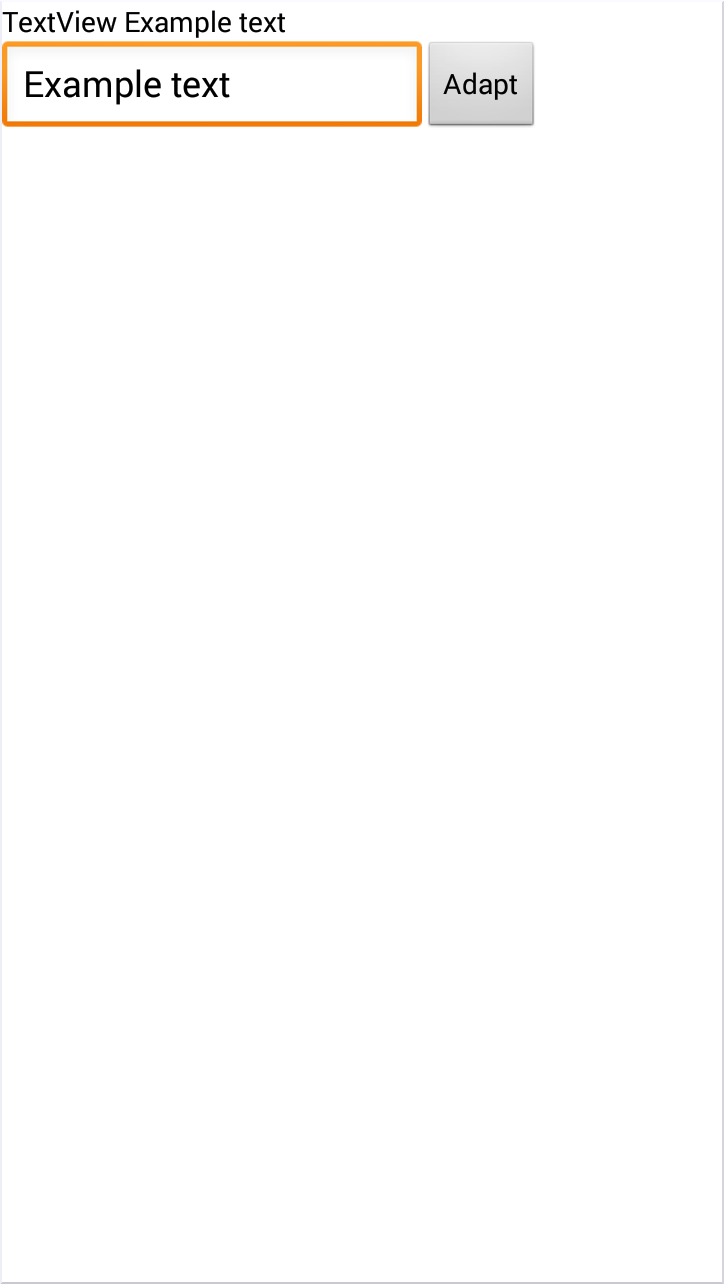
\includegraphics[width=0.25\textwidth]{default_layout.png}
\caption{The corresponding user interface considering the layout specified in
Listing~\ref{lst:default_layout}.}
\label{fig:default_layout}
\end{figure}

The usual Android code for managing the user interface is shown in Listing~\ref{lst:default_oncreate}.
Once the AdaptUI available adaptation methods are explained to the developers,
they are asked to make the mentioned user interface items dynamically adaptive.
The developers are asked to install the Capabilities Collector in their Android
devices. Then, they run it and they adapt the user interface as needed. After
the adaptation process (as users) they are asked to develop their own application,
showing a text view, an edit text, and a button. 

An example is shown in Listing~\ref{lst:adaptui_oncreate}. In it, it is shown 
how declaring an \textit{AdaptUI} object the adaptation of the views is easy and 
dynamic.

\inputminted[linenos=true, fontsize=\footnotesize, frame=lines]{java}{5_experiments_and_results/default_oncreate.java}
\captionof{listing}{The default \textit{onCreate} method.\label{lst:default_oncreate}}

\inputminted[linenos=true, fontsize=\footnotesize, frame=lines]{java}{5_experiments_and_results/adaptui_oncreate.java}
\captionof{listing}{The AdaptUI \textit{onCreate} method.\label{lst:adaptui_oncreate}}

Thus, the resulting adapted user interface is illustrated by Figure~\ref{fig:adapted_layout}.
While Figure~\ref{fig:default_layout} shows a default disposition and configuration
of the user interface items described in Listing~\ref{lst:default_layout}, in this
case they have been adapted according to Listing~\ref{lst:adaptui_oncreate}.

\begin{figure}
\centering
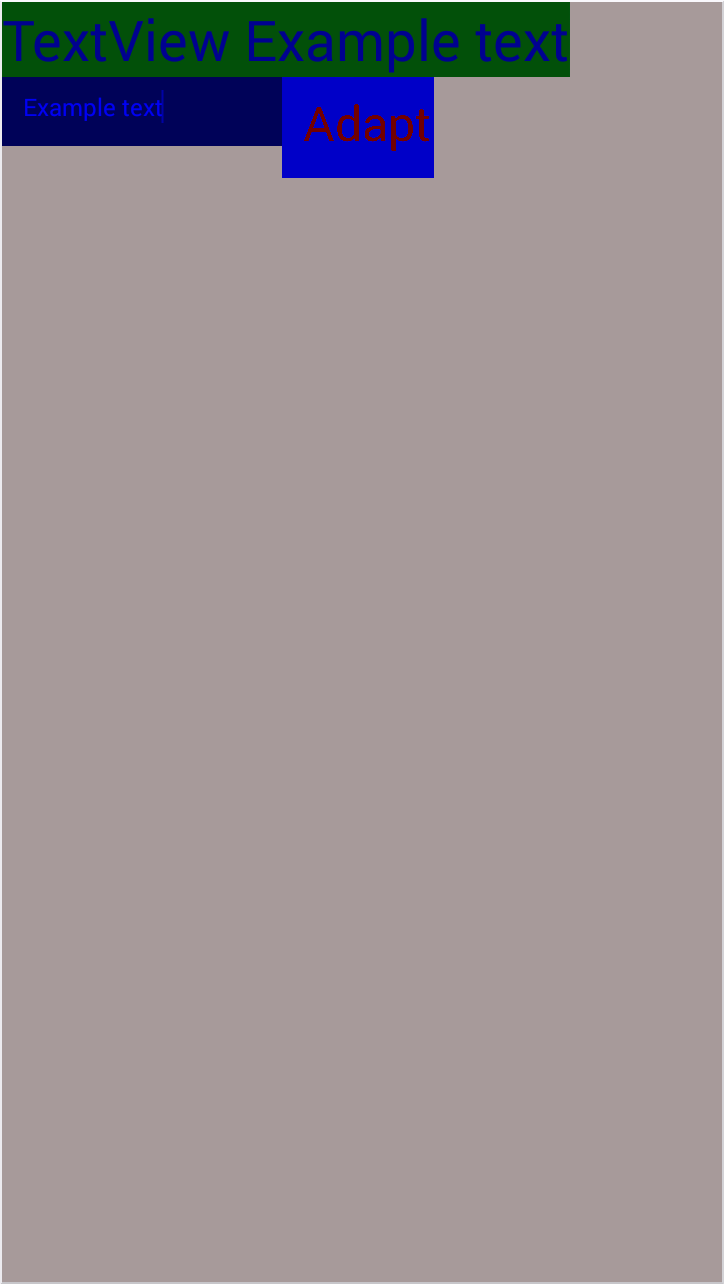
\includegraphics[width=0.25\textwidth]{adapted_layout.png}
\caption{The corresponding user interface considering the layout specified in
Listing~\ref{lst:adaptui_oncreate}.}
\label{fig:adapted_layout}
\end{figure}



\subsubsection{The knowledge editor \ac{api}}
\label{sec:knowledge_api}


%
\section{User Evaluation}
\label{sec:user_evaluation}

As said in the introduction of this chapter, this section deals with the user 
evaluation. In order to make a proper comparison between the presented systems 
several users have been guided through a demonstration of AdaptUI and a 
comparison with Imhotep. Besides, they have been questioned following the \ac{sus} 
guidelines.

\subsection{The \ac{sus} Questionnaire}
\label{sec:sus}
The \ac{sus} (System Usability Scale)~\citep{sus} is a 10-item questionnaire 
developed by John Brooke in 1986 which gives an overview of satisfaction of 
users with software. Originally, it was conceived as a ``quick and dirty'' 
scale to collect the usability feedback from using systems similar to VT100 
Terminal applications (see the DEC VT100 video terminal in 
Figure~\ref{fig:vt100}).

\begin{figure}
\centering
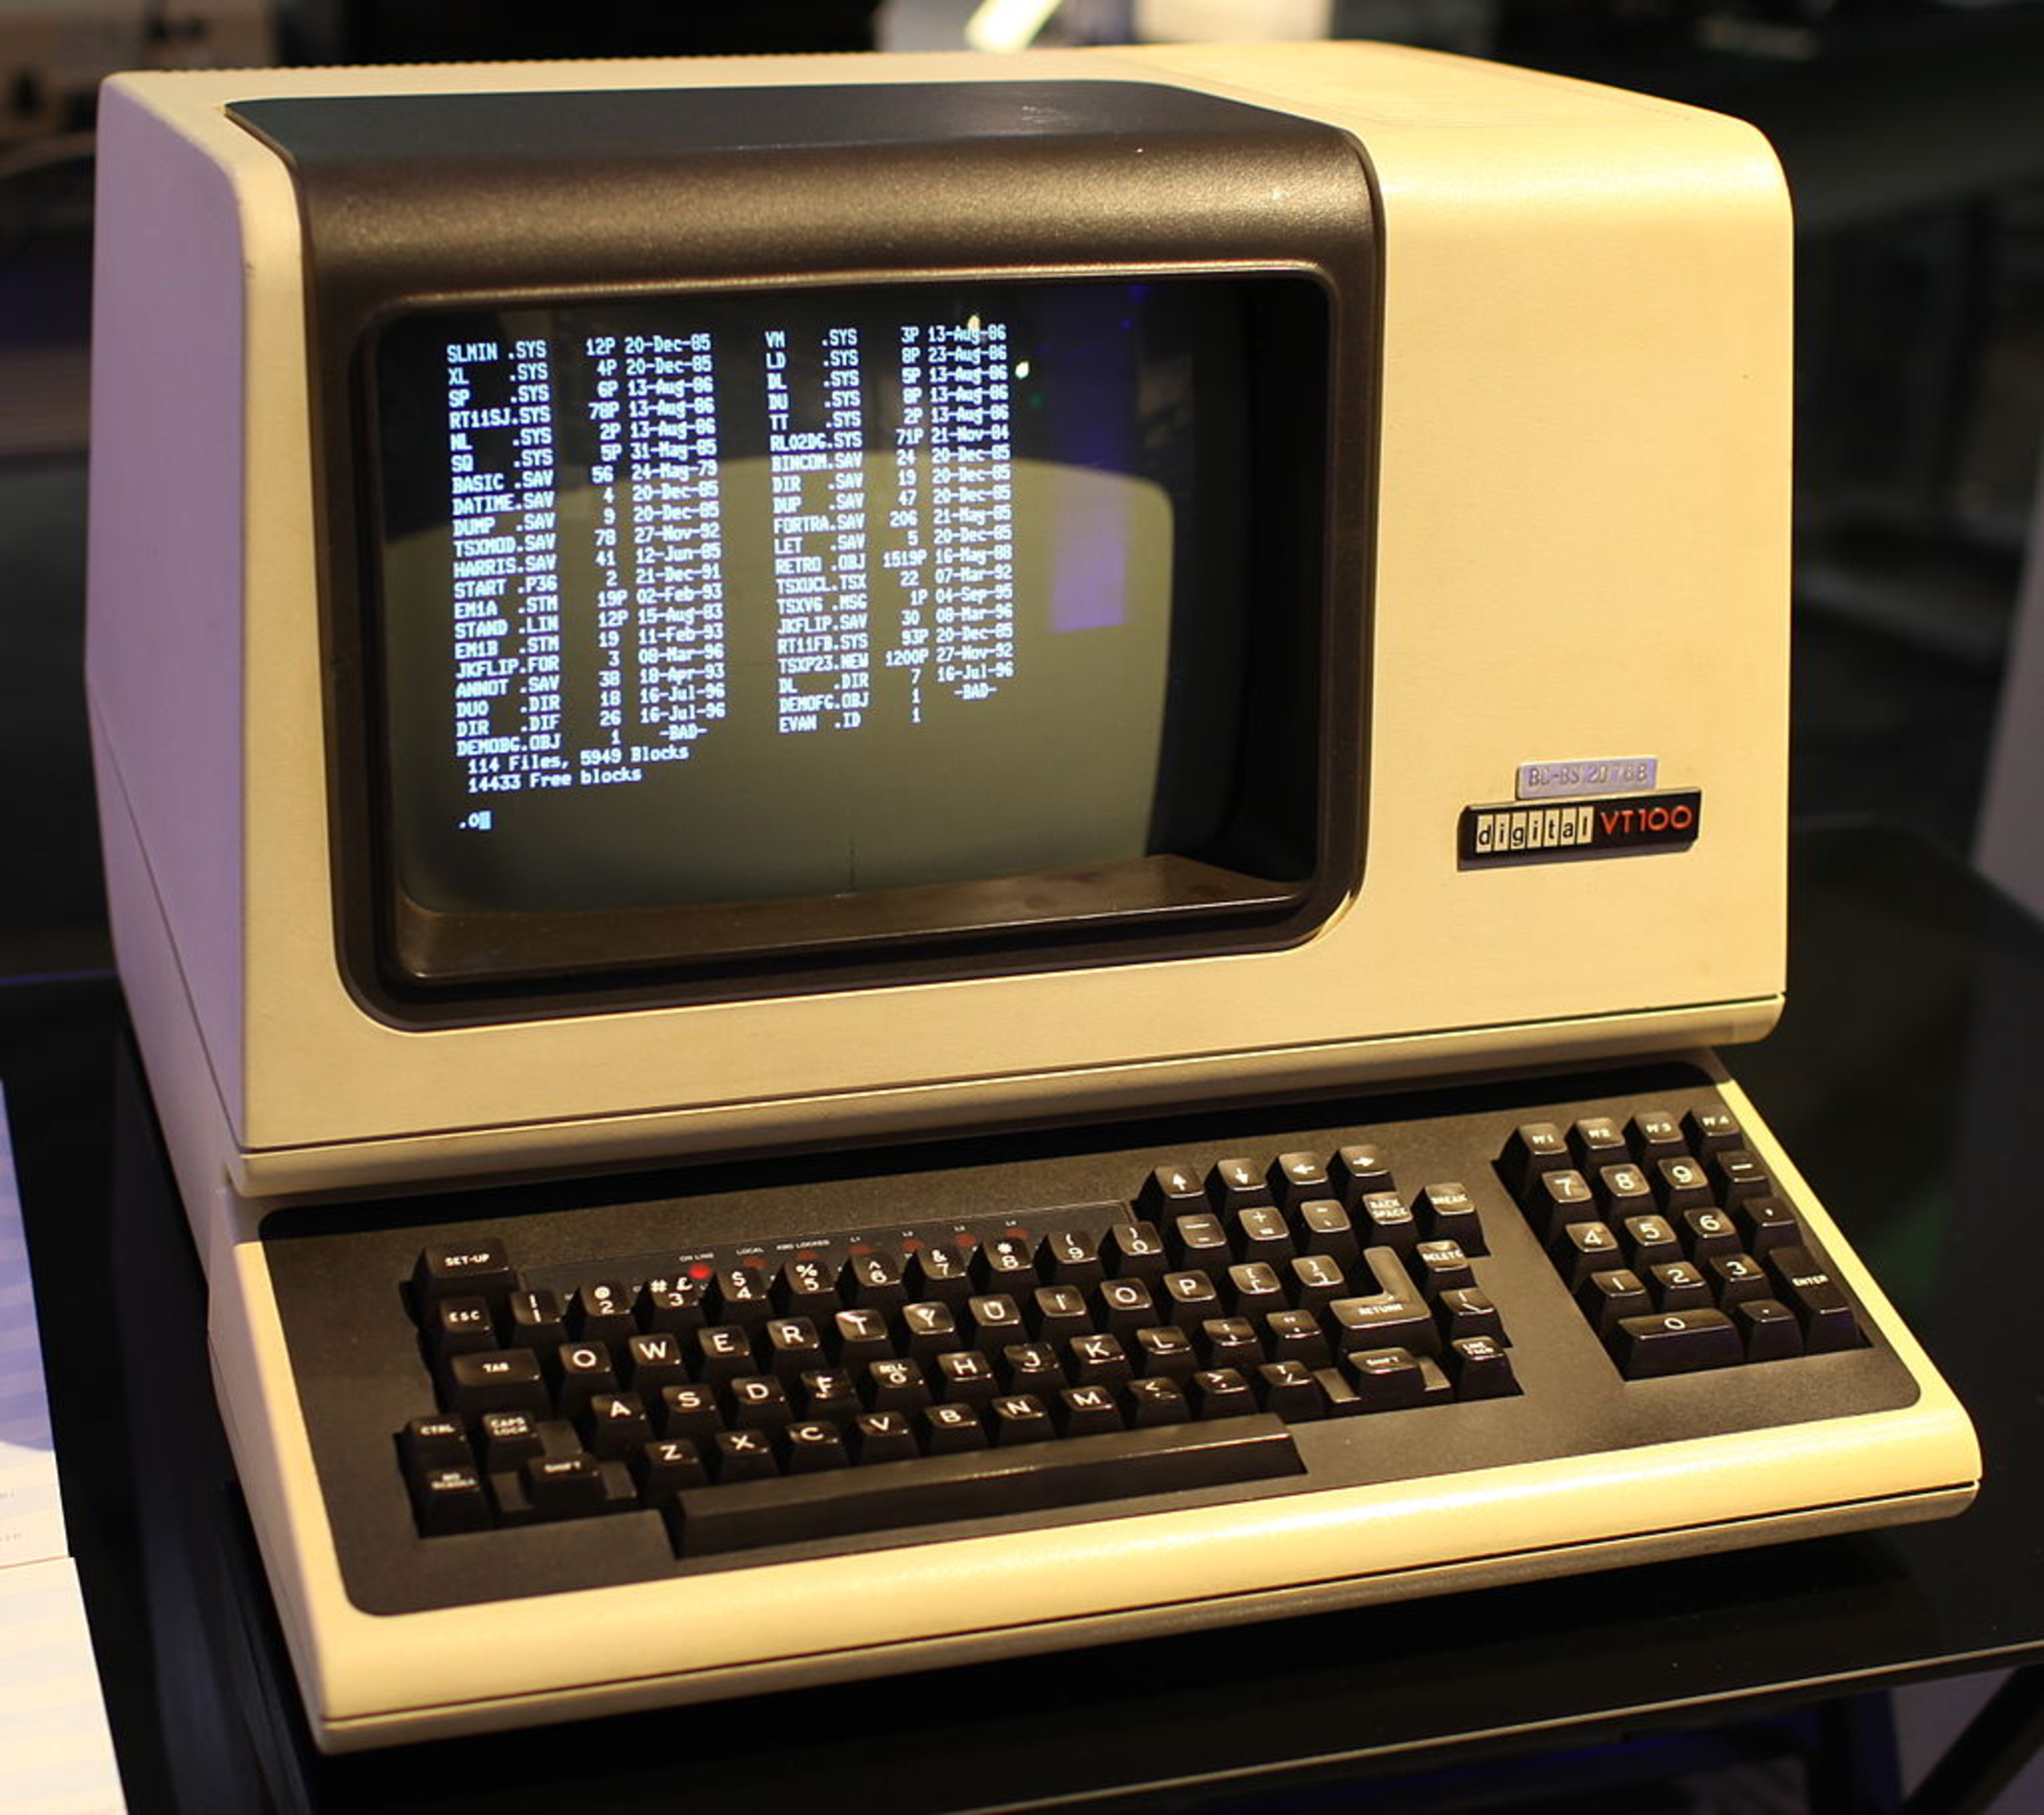
\includegraphics[width=0.65\textwidth]{vt100.pdf}
\caption{The Digital Equipment Corporation (DEC) VT100 video terminal, 
introduced in August 1978~\citep{vt100}.}
\label{fig:vt100}
\end{figure}

One of the \ac{sus} questionnaire main characteristics is its ability to collect
usability feedback through a 10 item questionnaire with 5 response options: 

\begin{enumerate}
 \item I think that I would like to use this system frequently.
 \item I found the system unnecessarily complex.
 \item I thought the system was easy to use.
 \item I think that I would need the support of a technical person to be able to
 use this system.
 \item I found the various functions in this system were well integrated.
 \item I thought there was too much inconsistency in this system.
 \item I would imagine that most people would learn to use this system very
 quickly.
 \item I found the system very cumbersome to use.
 \item I felt very confident using the system.
 \item I needed to learn a lot of things before I could get going with this
 system.
\end{enumerate}

To measure the resulting responses from the users, the formula described bellow
is applied: 

\begin{itemize}
 \item For odd items: subtract one from the user response.
 \item For even-numbered items: subtract the user responses from 5.
 \item This scales all values from 0 to 4 (with four being the most positive 
  response).
 \item Add up the converted responses for each user and multiply that total by 
  2.5. 
 This converts the range of possible values from 0 to 100 instead of from 0 to 
  40.
\end{itemize}

Thus, a figure between 0 and 100 is obtained, indicating the percentage of 
acceptance of the corresponding evaluated system. 
Figure~\ref{fig:sus_responses_example} shows an example of the \ac{sus} 
questionnaire format. Besides, Table~\ref{tbl:sus_results} shows an example of 
a completed \ac{sus} questionnaire evaluating a generic system. 

\begin{figure}
\centering
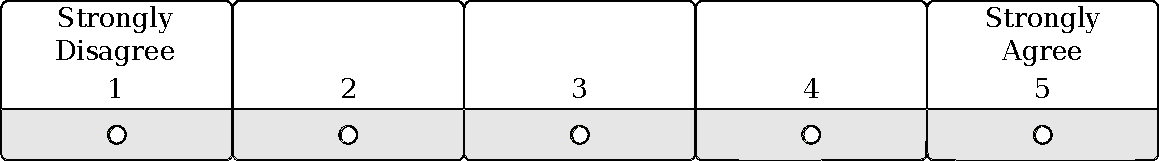
\includegraphics[width=0.65\textwidth]{sus_responses_example.pdf}
\caption{The \ac{sus} response format~\citep{vt100}.}
\label{fig:sus_responses_example}
\end{figure}


\begin{table}
 \caption{Example of a completed \ac{sus} questionnaire. Total score = 22;
 \ac{sus} Score = 22 * 22.5 = 55}
 \label{tbl:sus_results}
 \footnotesize
 \centering
\begin{tabular}{l c c c c c c}
  & \multicolumn{5}{c}{}\\
  & \begin{rotate}{60}\textbf{Strongly disagree}\end{rotate} & & & & 
\begin{rotate}{60}\textbf{Strongly agree}\end{rotate} \\
  \footnotesize
  1. I think that I would like to use this system frequently. 	& {\huge 
\Square} & {\huge \Square} & {\huge \Square} & {\huge \Square} & {\huge 
\CheckedBox}\\
  2. I found the system unnecessarily complex.& {\huge \Square} & {\huge 
\Square} & {\huge \Square} & {\huge \CheckedBox} & {\huge \Square}\\
  3. I thought the system was easy to use.& {\huge \Square} & {\huge 
\CheckedBox} & {\huge \Square} & {\huge \Square} & {\huge \Square}\\
  4. I think that I would need the support of a technical & {\huge \CheckedBox} 
& {\huge \Square} & {\huge \Square} & {\huge \Square} & {\huge \Square}\\
  person to be able to use this system. \\
  5. I found the various functions in this system were well & {\huge \Square} & 
{\huge \CheckedBox} & {\huge \Square} & {\huge \Square} & {\huge \Square}\\
  integrated. \\
  6. I thought there was too much inconsistency in this system.& {\huge \Square} 
& {\huge \Square} & {\huge \CheckedBox} & {\huge \Square} & {\huge \Square}\\
  7. I would imagine that most people would learn to use & {\huge \Square} & 
{\huge \CheckedBox} & {\huge \Square} & {\huge \Square} & {\huge \Square}\\
  this system very quickly. \\
  8. I found the system very cumbersome to use.& {\huge \Square} & {\huge 
\Square} & {\huge \Square} & {\huge \CheckedBox} & {\huge \Square}\\
  9. I felt very confident using the system.& {\huge \Square} & {\huge \Square} 
& {\huge \Square} & {\huge \Square} & {\huge \CheckedBox}\\
  10. I needed to learn a lot of things before I & {\huge \Square} & {\huge 
\Square} & {\huge \CheckedBox} & {\huge \Square} & {\huge \Square}\\
  could get going with this system. \\
\end{tabular}
\end{table}

Although there are other interesting questionnaires (i.e., \ac{sumi}~\citep{sumi},
\ac{mumms}~\citep{mumms}, \ac{quis}~\citep{quis}, and so on), the \ac{sus} 
questionnaire has become an industry standard with references in over 600 
publications~\citep{measuringusability}.

For this evaluation, and along with the \ac{sus} questionnaire, several extra 
questions have been added. The purpose of these questions is to segment the 
whole users set into different subsets of users under similar conditions. Thus, 
three extra classifications have been performed following the following 
criteria:

\begin{itemize}
  \item By age. The users of AdaptUI might encounter different difficulties when
  dealing with the adaptation platform. For example, users older than 65 may not
  be used to use smart devices or touching screens. As is shown through the 
  following charts, age and technology experience are related. To be aware of
  this issue an age based classification has been performed. The subgroups for
  this age classification are:
  \begin{itemize}
    \item Users aged under 20 years old ($x < 20$)\footnote{The $x$ represents
    the age of the user. In this case the $x$ is also shown in the following 
charts
    during this section in the Legend.}.
    \item Users aged between 20 and 35 years old ($20 \leq x < 35$).
    \item Users aged between 35 and 50 years old ($35 \leq x < 50$).
    \item Users aged between 50 and 65 years old ($50 \leq x < 65$).
    \item Users aged over 65 years old ($x > 65$).
  \end{itemize}

  \item By experience with technology. As it might happen with age, the 
  technology experience of the users might result into different usability 
  experiences when using AdaptUI. Touching screens, smart devices, or even 
  technical computer related instructions may be complex depending on the user 
  experience. Hence, a simple classification considering this problem is made 
  with the following criteria:
  
  \begin{itemize}
    \item Low, which indicates a user who is not very familiar with technology.
    This kind of users require non technical further explanations of the AdaptUI
    features, purpose and characteristics. Besides, several \ac{sus} questions might
    trouble these users. Thus, it is desirable to accompany them through the
    \ac{sus} process.
  
    \item Medium, which means that the user usually interacts with technology
    and understands the most common interaction processes and technical 
    vocabulary. Nevertheless, too technical instructions and features might 
    confuse them.
    
    \item High, which characterize those users who have high level technical
    knowledge due to their jobs, hobbies, age, and so forth. These users do not require
    extra explanations or guidelines.
  \end{itemize}
  
  \item By disability. Users are asked if they sense that they might suffer from
  visual or hearing disabilities. Problems when dealing with devices under 
  certain context conditions are included. On the contrary, no specific visual 
  or hearing disability is concreted. The idea is to capture the feeling of 
  the users when manipulating devices under certain conditions (due context 
  or due their own capabilities).
\end{itemize}

Hence, before beginning with the \ac{sus} questionnaire, the following 4 questions
are presented, allowing users to select the corresponding responses through
several combo boxes:

\begin{enumerate}[label=\alph*)]
  \item Please select your age within the following ranges.
  \item Which would you say your experience with technology level is?
  \item Do you feel that, sometimes, you cannot use your mobile device as you
  would like due to a temporary or enduring visual problem? This problem might
  be caused by physiological or context conditions.
  \item Do you feel that, sometimes, you cannot use your mobile device as you
  would like due to a temporary or enduring hearing problem? This problem might
  be caused by physiological or context conditions.
\end{enumerate}

Besides, after these and the \ac{sus} questions two extra questions are presented
regarding developers feedback. The responses are requested through several
check boxes:

\begin{enumerate}[label=\alph*)]
  \item I am a software developer and I usually work with user interfaces.
  \item Considering that I am a developer, I would find the AdaptUI \ac{api} very
  helpful to ease the adaptation of user interfaces.
\end{enumerate}


\subsection{Discussion}
\label{sec:user_evaluation_discussion}

After using AdaptUI and checking its adaptation capabilities, users have been 
asked to complete the \ac{sus} questionnaire with several extra questions. This 
test has been completed by a total of 30 users. Classified into different groups
regarding their age, technology experience and temporary or enduring disabilities 
the obtained results are explained in the following lines illustrated with several 
figures and charts.

First, without considering any of the cited classification criteria, the 
usability results regarding the AdaptUI adaptation system is illustrated through
Figure~\ref{fig:sus_responses}. This figure shows that the 69.56\% of the users
punctuated AdaptUI with over 70 within the \ac{sus} scale. On the contrary, 
approximately the 30\% of the users find its usability under 70 points.

\begin{figure}
\centering
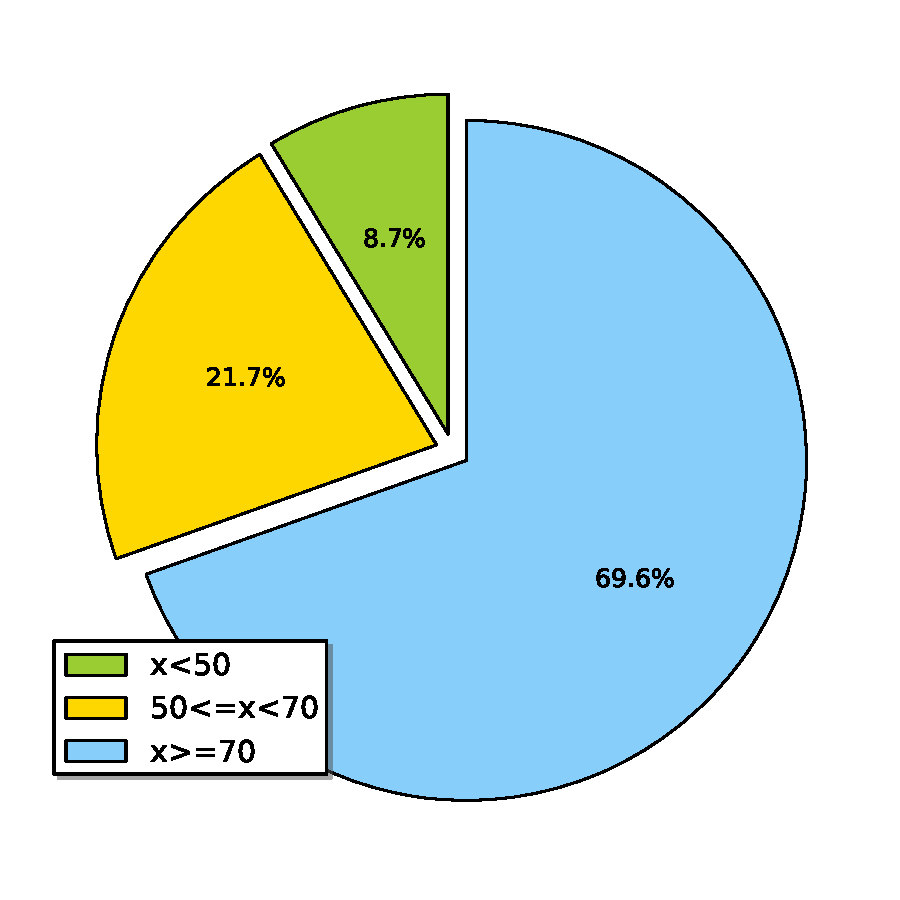
\includegraphics[width=0.65\textwidth]{sus_responses.pdf}
\caption{The \ac{sus} responses.}
\label{fig:sus_responses}
\end{figure}

Next, the cited criteria regarding age, technology experience and possible
disabilities result in the following bar charts. The Figure~\ref{fig:sus_age}
illustrates the differences regarding the \ac{sus} results taking into account the
users ages. In this chart is clearly shown how users between 20 and 35 years old
are the ones who mostly support the AdaptUI usability results. The 43.47\% of
these users consider that the usability of AdaptUI is over 70 in the \ac{sus} scale.

\begin{figure}
\centering
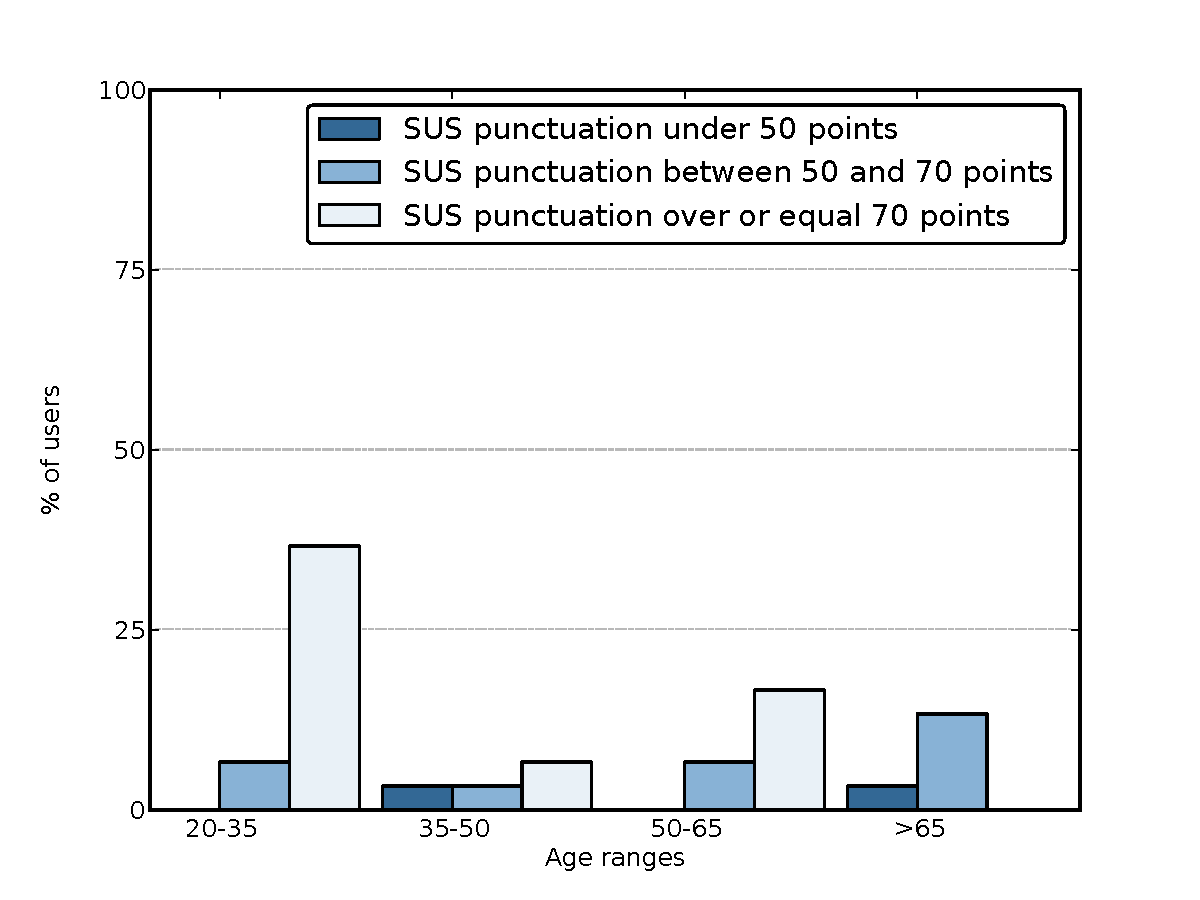
\includegraphics[width=0.65\textwidth]{sus_ages.pdf}
\caption{The \ac{sus} responses taking into account the age range of the users.}
\label{fig:sus_age}
\end{figure}

Along with the age, usually the experience with technology is directly related.
To have this into account, Figure~\ref{fig:sus_experience} illustrates the
resulting differences encountered after analysing the responses given to the \ac{sus}
questionnaire. As is shown, users with \textit{high} technology experience 
result into bigger usability results, reaching a final result of 43.47\% of 
users punctuating AdaptUI over 70 points in the \ac{sus} scale. On the opposite side 
there are those users who lack technology experience. The 8.69\% of these 
users gave less than 50 points. 

\begin{figure}
\centering
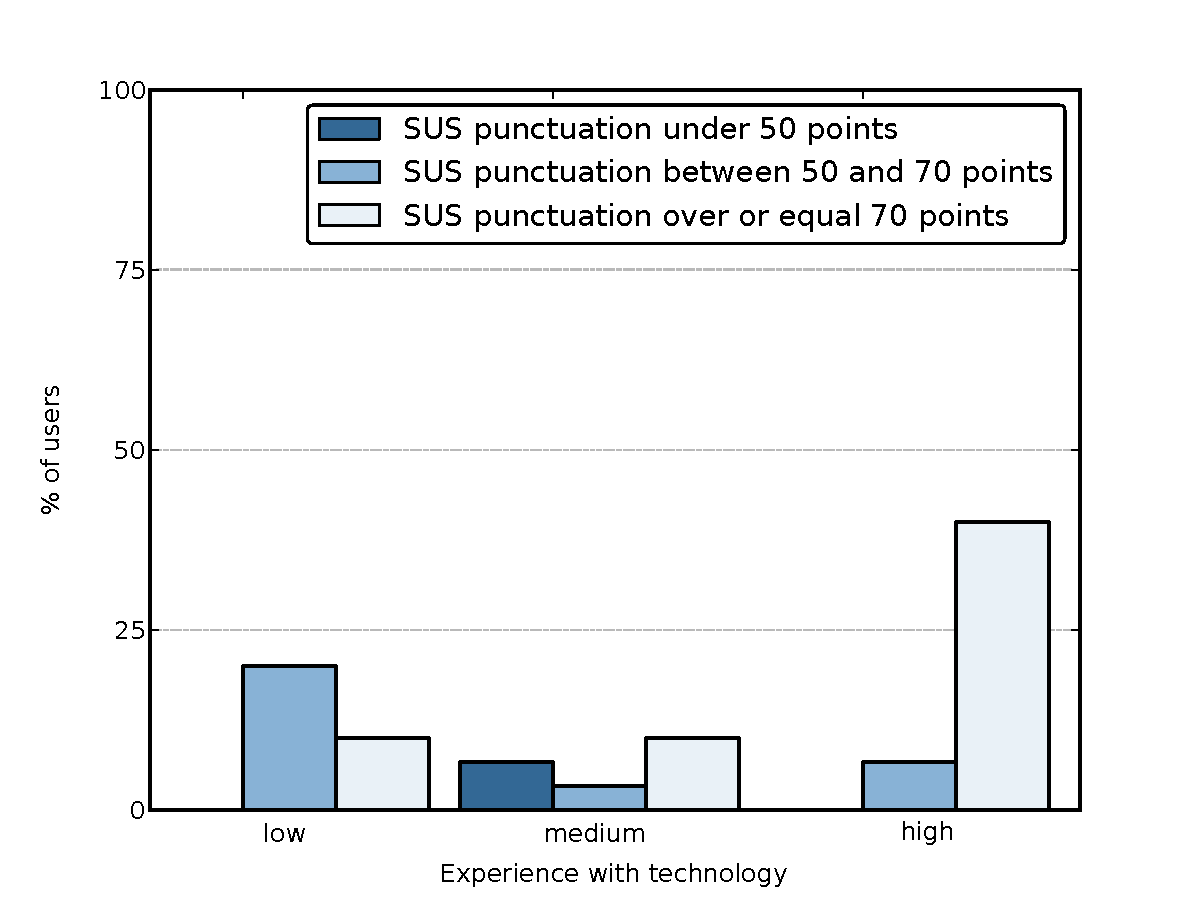
\includegraphics[width=0.65\textwidth]{sus_experience.pdf}
\caption{The \ac{sus} responses taking into account the experience with technology
of the users.}
\label{fig:sus_experience}
\end{figure}

Besides, users are asked about possible disabilities. These disabilities do not
have to be physiological. They are related with the feeling of disability that
users might sense, caused by the context under certain conditions or caused by
other factors. Every user is asked about any possible disability when dealing
with interaction with their devices. As AdaptUI does not consider physiological
capabilities, the users are not asked about this kind of issues directly. The
obtained results show how the 100\% of the asked users with visual or hearing
disabilities find AdaptUI totally usable, punctuating it in the \ac{sus} scale over
70.

\begin{figure}
\centering
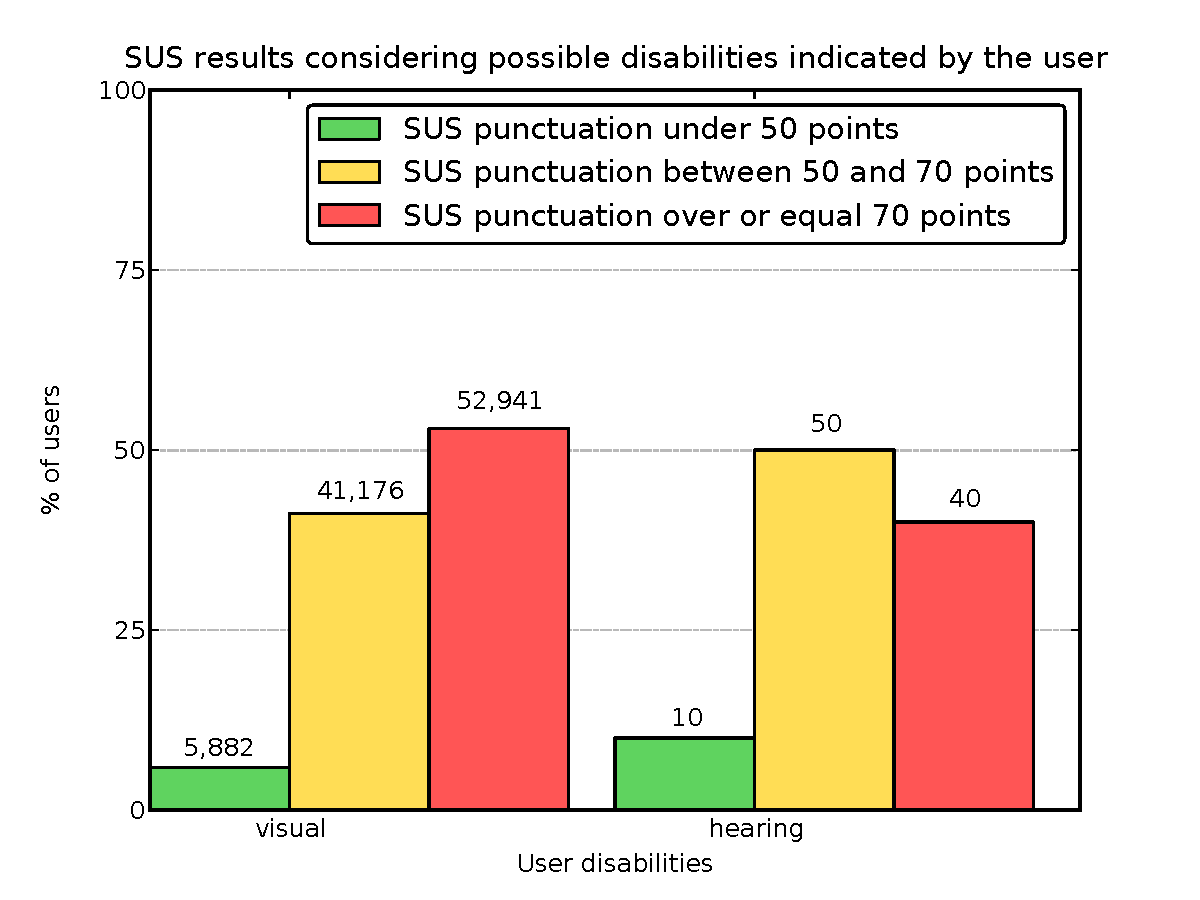
\includegraphics[width=0.65\textwidth]{sus_disability.pdf}
\caption{The \ac{sus} responses taking into account the visual and hearing 
disabilities
indicated by the users.}
\label{fig:sus_disability}
\end{figure}

Finally, we have distinguished between potential users and those who have
development knowledge. In the first versions of the questionnaire this was not
taken into account. However, several evaluations revealed that many users with 
developer profiles stated that they might not find AdaptUI useful as users. On
the contrary, they were willing to use it as developers due to the user 
interface adaptation capabilities of the platform. The 100\% of the users that 
consider themselves developers stated that they would like to use the platform. 
However, Figure~\ref{fig:sus_developers} shown how only the 66.67\% of these 
punctuate AdaptUI with a value of over 70 in the \ac{sus} scale. On the other side, 
the 22.22\% of the developers stated a value between 50 and 70.

\begin{figure}
\centering
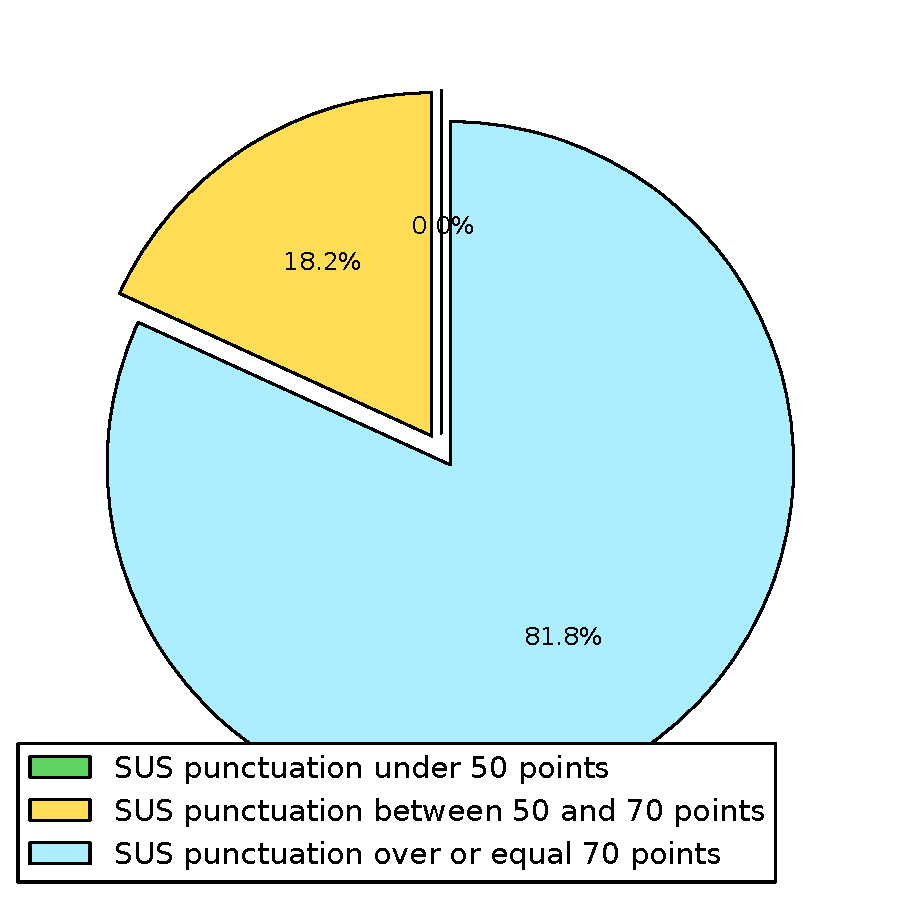
\includegraphics[width=0.65\textwidth]{sus_developers.pdf}
\caption{The \ac{sus} responses taking into account if users are developers.}
\label{fig:sus_developers}
\end{figure}

\subsection{Conclusions}
\label{sec:user_evaluation_conclusions}

Reviewing the results obtained during the user evaluation, several conclusions 
are extracted. In the following lines we summarize these conclusions taking into 
account the segmentation of users by age, experience with technology, possible 
or temporary disabilities, and developer users:

\begin{itemize}
  \item Users ageing is fundamental when dealing with AdaptUI for the first 
  time. While users under 35 years old seem very intuitive and understand most
  of the features and terminology easily, older users usually need more 
  high-level explanations. More precisely, the 43.47 of the users ageing between
  20 and 35 support AdaptUI with more than 70 points in the \ac{sus} scale. On the 
  contrary there are the users ageing over 65 years old. In this case, no one
  gave more than 70 points in the \ac{sus} scale. This is mostly because they 
  encountered several difficulties to understand not only the purpose of the
  system but also the features it provides, and the used and required 
  terminology. This is perceptible through Figure~\ref{fig:sus_age}.
  
  \item The experience with technology, highly associated with ageing, also 
  indicates more or less skill when using the AdaptUI system. Experienced users
  not only understand the features provided by AdaptUI, but they also predict
  the results of the experiments or even contribute with possible features to 
  cover they daily experiences with user interfaces. As is illustrated through
  Figure~\ref{fig:sus_experience}, the 43\% of the users with \textit{high} 
  experience with technology gave to AdaptUI more than 70 points in the 
  usability scale. Contrarily, the 8\% of the \textit{low} experienced users 
  the same punctuation.
  
  \item Regarding the possible disabilities we might suffer from when 
  manipulating our devices in different contexts, users are very comfortable 
  with the purpose of AdaptUI. Nevertheless, in this point we encountered 
  several differences. For example, a significant percentage of users that are
  also developers find the AdaptUI \ac{api} more interesting than the scenarios. 
  In other words, they prefer using AdaptUI as a framework for their applications
  than using it for their daily lives as mobile devices users. Focusing on the
  results, Figure~\ref{fig:sus_disability} shows similar outcomes considering
  both visual and hearing disabilities. In the first case the 63.63\% of the 
  users gave more than 70 points, while in the second case the percentage is 
  57.14\%.
  
  \item Finally, regarding the results obtained from users who are also 
  developers, we find that the 72.72\% of these users find AdaptUI usable, 
  giving 70 or more points in the \ac{sus} scale. The rest of developer users 
  stated that they find AdaptUI a necessary platform for the inclusive design of 
  the user interface of their applications, expressing that, as users (not 
  developers), they might not use AdaptUI. These outcomes are illustrated
  through Figure~\ref{fig:sus_developers}.
\end{itemize}

In general terms the acceptance of AdaptUI regarding usability and developer
needs is promising. As Figure~\ref{fig:sus_responses} shows, the 69.56\% of all 
the users find AdaptUI usable over 70 usability points. On the contrary only
the 8.69~\% gave less than 50 points. Nevertheless, and as is detailed in 
Section~\ref{sec:future_work}, more efforts are planned to try to get better
results for both users and developers.

\subsection{The \ac{sus} Results}
\label{sec:sus_results}
 
This section shows the results of the \ac{sus} questionnaire carried out among
30 potential users. Table~\ref{tbl:additional_questions} presents the replies 
to the additional questions detailed in Section~\ref{sec:sus}.
Table~\ref{tbl:sus_questionnaire_results} shows the anonymous responses and final
computed \ac{sus} value.

\begin{table}
  \caption{The additional questions.}
 \label{tbl:additional_questions}
\footnotesize
\centering
 \begin{tabular}{r l l l l l l}
  \hline 
  \textbf{\#User} & \textbf{Age range} 	& \textbf{Experience} & \textbf{Sight} & \textbf{Hearing} & \textbf{Developer} & \textbf{I find it} \\
		  &   			& 		      & \textbf{temporary}       & \textbf{temporary}	&	& \textbf{useful}\\
		  & 			& 		      & \textbf{disability}	 & \textbf{disability} & & \\
  \hline
  $\#1$ & $20-35$ 	     & High		   & No			      & No			   & No			& No	\\
  $\#2$ & $20-35$ 	     & Medium		   & Yes		      & Yes			   & No			& No	\\
  $\#3$ & $20-35$ 	     & High		   & No			      & No			   & Yes		& Yes	\\
  $\#4$ & $20-35$ 	     & High		   & No			      & No			   & Yes		& Yes	\\
  $\#5$ & $20-35$ 	     & High		   & No			      & No			   & Yes		& Yes	\\
  $\#6$ & $51-65$ 	     & Medium		   & No			      & No			   & No			& No	\\
  $\#7$ & $20-35$ 	     & High		   & No			      & No			   & Yes		& Yes	\\
  $\#8$ & $20-35$ 	     & High		   & No			      & No			   & Yes		& Yes	\\
  $\#9$ & $20-35$ 	     & High		   & No			      & No			   & Yes		& Yes	\\
  $\#10$ & $20-35$ 	     & High		   & No			      & No			   & Yes		& Yes	\\
  $\#11$ & $20-35$ 	     & High		   & No			      & No			   & Yes		& Yes	\\
  $\#12$ & $20-35$ 	     & High		   & No			      & No			   & Yes		& Yes	\\
  $\#13$ & $20-35$ 	     & High		   & Yes		      & No			   & Yes		& Yes	\\
  $\#14$ & $51-65$ 	     & Low		   & Yes		      & Yes			   & No			& No	\\
  $\#15$ & $51-65$ 	     & Low		   & Yes		      & No			   & No			& No	\\
  $\#16$ & $20-35$ 	     & High		   & Yes		      & No			   & No			& No	\\
  $\#17$ & $>65$ 	     & Medium		   & No			      & No			   & No			& No	\\
  $\#18$ & $36-50$ 	     & High		   & Yes		      & No			   & Yes		& No	\\
  $\#19$ & $51-65$ 	     & Medium		   & Yes		      & Yes			   & No			& No	\\
  $\#20$ & $51-65$ 	     & Low		   & Yes		      & Yes			   & No			& No	\\
  $\#21$ & $36-50$ 	     & Low		   & Yes		      & Yes			   & No			& No	\\
  $\#22$ & $36-50$ 	     & Medium		   & Yes		      & Yes			   & Yes		& Yes	\\
  $\#23$ & $>65$	 	     & Low		   & Yes		      & Yes			   & No			& No	\\
  \hline
\end{tabular}
\end{table}

The \ac{sus} questions are the following:
\begin{enumerate}
  \item \#Q1: I think that I would like to use this system frequently.
  \item \#Q2: I found the system unnecessarily complex.
  \item \#Q3: I thought the system was easy to use.
  \item \#Q4: I think that I would need the support of a technical person to be 
  able to use this system.
  \item \#Q5: I found the various functions in this system were well integrated.
  \item \#Q6: I thought there was too much inconsistency in this system.
  \item \#Q7: I would imagine that most people would learn to use this system 
  very quickly.
  \item \#Q8: I found the system very cumbersome to use.
  \item \#Q9: I felt very confident using the system.
  \item \#Q10: I needed to learn a lot of things before I could get going with 
  this system.
\end{enumerate}

\begin{table}
  \caption{Results of the \ac{sus} questionnaire.}
 \label{tbl:sus_questionnaire_results}
\footnotesize
\centering
 \begin{tabular}{r r r r r r r r r r r r}
  \hline 
  \textbf{\#User} &\textbf{\#Q1} & \textbf{\#Q2}& \textbf{\#Q3}& \textbf{\#Q4}& \textbf{\#Q5}& \textbf{\#Q6}& \textbf{\#Q7}& \textbf{\#Q8}& \textbf{\#Q9} & \textbf{\#Q10} & \textbf{Total}\\
    \hline
  $\#1$ & 4	& 2& 	4& 	1& 	4& 	2& 	4& 	1& 	5& 	1& 85\\
  $\#2$ & 5&	2&	4&	2&	3&	3&	5&	2&	4&	1& 77.5\\
  $\#3$ & 4&	3&	4&	4&	4&	2&	4&	2&	4&	4& 62.5\\
  $\#4$ & 2&	1&	4&	1&	4&	2&	3&	1&	4&	1& 77.5\\
  $\#5$ & 5&	2&	4&	2&	4&	3&	4&	1&	4&	2& 77.5\\
  $\#6$ & 5&	1&	5&	4&	5&	1&	5&	1&	3&	3& 82.5\\
  $\#7$ & 2&	1&	4&	1&	5&	1&	3&	1&	5&	1& 85\\
  $\#8$ & 3&	2&	5&	3&	4&	2&	5&	2&	4&	4& 70\\
  $\#9$ & 3&	1&	5&	1&	4&	2&	4&	1&	5&	1& 87.5\\
  $\#10$ & 2&	2&	4&	1&	4&	2&	4&	1&	5&	1& 80\\
  $\#11$ & 3&	2&	3&	1&	3&	1&	2&	2&	2&	2& 62.5\\
  $\#12$ & 4&	1&	4&	2&	4&	1&	3&	1&	4&	1& 82.5\\
  $\#13$ & 4&	1&	5&	1&	4&	1&	5&	1&	5&	1& 95\\
  $\#14$ & 4&	1&	5&	3&	5&	1&	5&	1&	2&	3& 80\\
  $\#15$ & 5&	3&	3&	4&	5&	3&	3&	2&	2&	2& 60\\
  $\#16$ & 4&	1&	5&	2&	4&	2&	4&	1&	5&	1& 87.5\\								
  $\#17$ & 1&	3&	2&	3&	3&	3&	1&	3&	5&	4& 40\\
  $\#18$ & 5&	1&	5&	3&	3&	2&	3&	2&	4&	1& 77.5\\
  $\#19$ & 4&	1&	4&	4&	5&	1&	5&	1&	3&	3& 77.5\\
  $\#20$ & 5&	2&	4&	5&	5&	1&	5&	1&	2&	3& 72.5\\
  $\#21$ & 4&	2&	3&	4&	4&	3&	5&	3&	3&	4& 57.5\\
  $\#22$ & 2&	3&	3&	3&	2&	3&	2&	2&	3&	2& 47.5\\
  $\#23$ & 4&	2&	3&	4&	5&	3&	5&	4&	3&	5& 55\\

  \hline
\end{tabular}
\end{table}
% 
\section{Evaluation Discussion}
\label{sec:evaluation_discussion}

Along this chapter several experiments have been carried out to test the AdaptUI
platform. First, we have compared the possible consequences of porting semantics
and reasoning to a mobile Android based platform. Through the experiments shown 
in Section~\ref{sec:technical_evaluation} it has been demonstrated how managing 
semantics in mobile phones is possible and affordable. The only condition we 
find that should be considered when dealing with mobile reasoning is that the 
ABox and \ac{swrl} axioms set should be limited or small enough to avoid the 
overloading of the whole system. Table~\ref{tbl:eval_default_ont},
Table~\ref{tbl:eval_abox} and Table~\ref{tbl:eval_swrl} show these differences 
remarking performance of reasoning for the corresponding execution platform.

After this first part of the experiments, a comparison between other 
alternatives has been presented. As is explained in 
Section~\ref{sec:imhotep_vs_adaptui}, Imhotep is a framework which aims to ease 
the development of adaptive user interfaces. The main problems or limitations 
of the Imhotep framework are: 

\begin{itemize}
  \item It cannot be deployed in a mobile phone. The design of the platform
  requires the existence of an external server which will manage the adaptation.
  
  \item To collect the user profile and capabilities a client application in
  the user's mobile phone is needed. This application sends user and device
  profile to the adaptation server.
  
  \item Besides, the knowledge about the user capabilities is physiological,
  which we have defended along this dissertation to be non practical and 
difficult
  to manage.
  
  \item It does not consider the current context, limiting the adaptations
  to the user's and devices capabilities.
  
  \item The adaptations are static. Once the server compiles the corresponding
  sources and the user interfaces are adapted, if the user is not comfortable
  with them the whole process has to be repeated.
  
  \item Finally, there is the problem of the network dependency, which 
  approximately adds 14 seconds to the whole process for compiling the 
  corresponding sources. Although Imhotep's performance when using the cache is 
  good enough (see Figure~\ref{fig:imhotep_comparison}), the response time 
  decreases significantly  when this cache is not present.
\end{itemize}


AdaptUI faces these problems inherited from Imhotep and solve them as follows:

\begin{itemize}
  \item Regarding the problem of using an external server, the AdaptUI platform
  runs fully in the mobile device. It is true that nowadays these devices'
  capabilities are far from the ones present when Imhotep was conceived. This
  allowed us to design a platform compatible with Android and network or 
  external services independent. Through the ontology and several optimized 
  adaptation engines the adaptation is carried out without needing external 
  processing assistance.
  
  \item Although AdaptUI also requires a software module to collect user
  capabilities, the perspective differs. In AdaptUI, the Capabilities Collector
  module aims to collect user capabilities regarding their preferences, not
  the physiological capabilities themselves. Besides, this module is fully
  integrated in the AdaptUI platform.
  
  \item As said before, AdaptUI does not consider physiological capabilities of
  the user. Instead of that, AdaptUI looks for several preferences of the user,
  modelled through the AdaptUIOnt ontology. Thus, adaptations and corrections
  on the corresponding adaptations are easier and practical.
  
  \item Regarding the context issue, AdaptUI considers the environment as one 
  of the three main entities in the user interfaces adaptation domain. Besides,
  the disabilities that users might suffer are understood as a set of conditions
  that somehow limit the user. These conditions do not have to be specifically
  physiological. To us, context might also generate several situations in which
  the user might feel temporary disabled.
  
  \item The adaptations are dynamic, not just considering that they are 
  modifiable in running time. They also change according to the experience 
  monitored by the Adaptation Polisher. This module aims to always monitor the 
  user interaction with the adapted interfaces to provide alternatives if the 
  usability decreases.
  
  \item AdaptUI does not depend on any network connection. It runs fully in the
  mobile device, which allows a complete independence from external connectivity
  issues.
\end{itemize}

Regarding the performance of both platforms, Table~\ref{tbl:imhotep_vs_adaptui}
shows how after loading the ontology, the adaptation process response in AdaptUI
is acceptable, not exceeding 2 seconds. On the contrary, if the cache is not
used, Imhotep has to deal with a performance over 14 seconds due to the network
dependency.


After these comparisons, several qualitative experiments have been presented 
through different scenarios (see Section~\ref{sec:scenarios}). These experiments 
are based on several complex situations, in which AdaptUI is scrutinized.
The presented scenarios have been categorized into 3 different groups, each 
group representing a concrete situation in which an adaptation of the user 
interface would be needed. In this case, these categories are:

\begin{enumerate}[label=\alph{*}]
  \item Limitations caused by the context current conditions.
  \item Limitations caused by the set of activities the user might be doing.
  \item Limitations caused by the disabilities the user might suffer from.
\end{enumerate}

These scenarios present a series of characteristics that distinguish them. After
analysing each specific situation, the adaptation process is detailed. Besides,
before presenting several conclusions, this adaptation process performed by 
AdaptUI is compared with Imhotep. Thus, an overview of the behaviour and 
performance of both systems is depicted.

Finally, the users' feedback is collected. To do so, an experiment with AdaptUI 
has been developed. Users have to use an application which translates the 
interaction to the AdaptUIOnt ontology. Then, several context changes are 
triggered so that the users see how the user interface adapts dynamically. After 
this experiment, a questionnaire is presented, so their experiences with the 
AdaptUI platform can be collected. Along with several extra questions to ease 
the analysis of the results, the \ac{sus} questionnaire is used. The main idea 
extracted from these results is that users find the platform useful. Although 
there are several differences considering one group of users or another (e.g., 
based on their age, technical experience or disability), the obtained results 
are promising. Besides, the requested developers also consider that the 
framework would benefit from the design of adaptive user interfaces, integrating 
them with their personal applications. Hence, we conclude that, although much work 
can be performed, the results of the evaluation performed and described in this 
chapter are promising.
\section{Conclusions}
\label{sec:evaluation_conclusions}

During this dissertation we have introduced AdaptUI as a platform for dynamic
user interface adaptation. As new technical contributions have been developed 
and detailed (e.g., a mobile reasoning engine), several experiments regarding 
this area have been presented. Comparing the presented system with others gives
us the perspective to criticise AdaptUI and extract several conclusions. In this
section these conclusions are depicted.

On the one hand, the performed technical experiments revealed that mobile 
reasoning engines are useful, practical and affordable regarding performance. It
is true that, in this case \textit{Pellet4Android} suffers depending on the 
hardware of the device. Besides, the more axioms we add to the corresponding 
ontology (specially to the \ac{swrl} axioms set), the more delay in the performance 
of the system is added. However, we believe that the AdaptUIOnt ontology is 
light enough to be easily managed by any Android based device. Furthermore, the 
smartphones market is increasing the possibilities of these devices by 
improving their hardware capabilities. This means that in the near future 
complex processing will be totally affordable by these devices. 

The comparison with Imhotep exposes several benefits of AdaptUI. The first one, 
is the lack of dependency on external services or servers. This fact does not 
only have an affect on the performance, it avoids possible network failure 
problems. Another fundamental aspect that should be emphasized due to this 
comparison is the way users are modelled. While in Imhotep specific user 
disabilities are needed, AdaptUI just requires a simple interaction with the 
Capabilities Collector module. The interaction of the user is translated to the 
AdaptUIOnt ontology, and the rest of the adaptation process is delegated to the 
AdaptUI platform. Besides, AdaptUI relies on the Adaptation Polisher to perform
slight modifications on the fly of the adapted user interface, in case the 
interaction with the user is not satisfactory. Regarding the time 
performances, although using cached applications in Imhotep shown a faster 
response, the truth is that regarding new and real scenarios revealed a much 
bigger accuracy in AdaptUI. This has been shown through the scenarios presented 
in Section~\ref{sec:scenarios}.

On the other hand XX users have tested the platform and have been asked about 
its usability. Users seem to react satisfactorily to AdaptUI. The obtained 
results through the questionnaire show how depending on the users ageing and 
technical knowledge they feel more or less comfortable with it. These results
also exposes how most developers would use it as a tool for their applications, 
but not as users. On the contrary, users who declare to suffer sometimes from
context disabilities are willing to use it integrated with their Android device.

% 
% As we aimed to evaluate not only the technical specifications of AdaptUI wee 
% studied how we could include the user feedback in the whole evaluation equation.
% In order to do this, a demonstrator has been developed under a controlled 
% environment to collect this feedback through a usability questionnaire.
% 
% After analysing the results obtained during the experiments presented in this 
% chapter, the following conclusions are noted:
% 
